\documentclass[a4paper,11pt,twoside]{IT-CNEA}
\usepackage[utf8]{inputenc} % para cambiar el encoding
\usepackage{multicol}

%%%%%%%%%%%%%%%%%%%%%%%%%%%%%%%%%%%%%%%%%%%%%%%%%%%%%%%%%%%%%%%%%%%%%%%%%%%
%               Parametros principales del documento                      %
%%%%%%%%%%%%%%%%%%%%%%%%%%%%%%%%%%%%%%%%%%%%%%%%%%%%%%%%%%%%%%%%%%%%%%%%%%%

% Titulo
\titulo{Propagación de ruido en sistema LTI}
%
% Titulo alternativo para el encabezado
\alttitulo{Elementos de matemáticas aplicada para aplicaciones tecnlógicas}

% Autores
\autores{Augusto Conrado Sardá}{}

% Revisores
\revisores{Jose Relloso}{Agustín Casquero}{}

% Revision de calidad
\calidad{}

% Aprobacion
\aprobacion{}

%Objetivo
\objetivo{}
% Alcance
%\alcance{}

% Numero de informe tecnico
\numeroIT{TP Nº0}
% Metadatos para pdf
\hypersetup{
    pdfauthor={Augusto Conrado Sardá},
    pdftitle={Propagación de ruido en sistema LTI},
    pdfkeywords={},
    pdfcreator={},
    pdfsubject={}    
    }
    
% Autores de revisiones
%\definechangesauthor[name={Johann Sebastian Mastropiero}, color=blue]{mas}
\usepackage{units}
\usepackage{fancyvrb}
\begin{document}
    % Creacion de la caratula
%    \portada    
    % Creacion del indice
    \tableofcontents       
    % Comienzo del desarrollo del documento
    \printnomenclature[2cm]

\newpage  
\section{INTRODUCCIÓN}
Los sistemas de navegación inerciales son capaces de proveer la posición, velocidad y actitud con
gran exactitud sobre cortos períodos de tiempo. Sin embargo, esta exactitud se degrada a medida que el
tiempo transcurre. Los requerimientos para una estimación exacta de la información para la navegación
requiere modelar los errores del sensor.
\par \textit{Allan variance} (AV) es la manera más simple de realizar este modelado. AV es un método para
representar el valor cuadrático medio (RMS) del error en función del tiempo promedio.
AV presenta la ventaja que es simple de calcular y analizar. Realizando operaciones sencillas a lo largo
de un conjunto de datos de la lectura de un sensor inercial, se obtiene una curva que permite caracterizar varios
errores aleatorios característicos de este tipo de sensores.
\section{ALLAN VARIANCE}

Supóngase que se tienen $N$ valores de la lectura de velocidad angular $\Omega$ de un sensor inercial que fueron muestreados con un período de muestreo $t_0$. A partir de este conjunto de datos, se forman subconjuntos de $n$ elementos (con $n<N/2$). El tiempo asociado a cada subconjunto es $T=nt_0$. El promedio $\bar{\Omega}$ es
\begin{equation}
\bar{\Omega}_k(T)=\frac{1}{T}\int_{t_k}^{t_k+T}\Omega(t)dt
\label{ec:velAngPromk}
\end{equation}
El promedio del siguiente subconjunto es
\begin{equation}
\bar{\Omega}_{next}(T)=\frac{1}{T}\int_{t_{k+1}}^{t_{k+1}+T}\Omega(t)dt
\label{ec:velAngPromSig}
\end{equation}
donde $t_{k+1}=t_k+T$. Luego, se define ``el'' Allan variance como
\begin{equation}
\sigma^2(T)=\frac{1}{2\left( N-2n\right)}\sum_{k=1}^{N-2n}\left[\bar{\Omega}_{next}(T)- \bar{\Omega}_k(T)\right]^2
\label{ec:AVVelAngular}
\end{equation}
Otra manera de calcular Allan variance es utilizar la posición angular en lugar de la velocidad angular. Para esto, se debe integrar esta última puesto que es la lectura del sensor
\begin{equation}
\theta(t)=\int^t\Omega(\xi)d\xi
\end{equation}
donde $\xi$ es una variable de integración. El límite inferior de la integral no se especifica ya que se utilizan las diferencias de velocidad angular. Las Ec.(\ref{ec:velAngPromk}) y Ec.(\ref{ec:velAngPromSig}) resultan ahora
\begin{equation}
\bar{\Omega}_{k}(T)=\frac{\theta_{k+n}-\theta_k}{T}
\end{equation}
\begin{equation}
\bar{\Omega}_{next}(T)=\frac{\theta_{k+2n}-\theta_{k+n}}{T}
\end{equation}
Reemplazando en la Ec.(\ref{ec:AVVelAngular})
\begin{equation}
\sigma^2(T)=\frac{1}{2T^2\left( N-2n\right)}\sum_{k=1}^{N-2n}\left[ \theta_{k+2n}-2\theta_{k+n}+\theta_k \right]^2
\label{ec:AVPosAngular}
\end{equation}
\par En los sensores inerciales se conoce cuales son algunas de las fuentes características de ruido. Los cinco más básicos son: quantization noise, angle random walk, bias instability, rate random walk y drift rate ramp\footnote{No se los traduce al español por la costumbre de emplear estos términos en inglés}. Cada una de estas componentes de ruido está caracteriza por su función de densidad espectral de frecuencia (PSD) $S_{\Omega}(f)$. La relación de esta con $\sigma^2(T)$  es
\begin{equation}
\sigma^2(T)=4\int_0^{\infty}S_{\Omega}(f)\frac{\sin^4(\pi fT)}{\left( \pi fT\right)^2}df
\label{ec:relacionPSDAV}
\end{equation}
Las hipótesis requeridas sobre la Ec.(\ref{ec:relacionPSDAV}) es que el proceso aleatorio $\Omega(t)$ sea estacionario. Esto implica que la función de autocorrelación $\Omega(t)$ no depende del tiempo y que sea par.
\\ La Ec.(\ref{ec:relacionPSDAV}) establece que $\sigma^2(T)$ es proporcional a la potencia de salida de la señal aleatoria $\Omega(t)$ al pasar por un filtro con función transferencia de la forma $\sin^4(x)/x^2$. Esta función transferencia es consecuencia del método empleado para crear y operar los subconjuntos. 
\\ En la Ec.(\ref{ec:relacionPSDAV}) se encuentra la principal ventaja del método de AV. Por un lado, si se conoce la PSD de cualquier proceso aleatorio, se puede conocer como debe ser su AV. En sentido opuesto, dado que $\sigma(T)$ se puede calcular a partir de mediciones de un sensor (Ec.(\ref{ec:AVPosAngular})) se crea un gráfico de AV y se puede inferir información sobre el proceso aleatorio.
\\ La Ec.(\ref{ec:relacionPSDAV}) también manifiesta que el ancho de banda del filtro depende del tiempo $T$ del subconjunto. De esta manera, se pueden examinar distintos tipos de procesos aleatorios variando $T$ (para así variar el ancho de banda). Por lo tanto, AV permite identificar y cuantificar diferentes tipos de errores presentes en las mediciones del sensor. 
\subsection{REPRESENTACIÓN DE TÉRMINOS DE RUIDOS EN ALLAN VARIANCE}
\subsection{QUANTIZATION NOISE}
Es un error que se produce al digitalizar una señal analógica. Es causado por las pequeñas diferencias entre los valores reales de la señal siendo muestrada y la resolución del conversor analógico digital.
\\ Para la salida de un giróscopo, la PSD de la posición angular es
\begin{equation}
S_{\theta}=T_sQ_z^2\left[ \frac{\sin\left( \pi ft\right)}{\pi ft}\right]^2\approx T_sQ_z^2\,;\,f<\frac{1}{2T_s}
\end{equation}
donde $T_s$ es el período de muestreo y $Q_z$ es el coeficiente de quantization noise. El límite teórico para $Q_z$ es $S/\sqrt{12}$, donde $S$ es el coeficiente de escala del giróscopo en pruebas con tiempo de muestreo fijo y uniforme.
\\ La relación entre la PSD de la velocidad angular y la de la posición angular es 
\begin{equation}
S_{\Omega}=\left( 2\pi f\right)^2S_{\theta}\left( 2\pi f\right)\approx 	\left( 2\pi f\right)^2T_sQ_z\,;\,f<\frac{1}{2T_s}
\label{ec:PSDQuantization}
\end{equation}
Reemplazando la Ec.(\ref{ec:PSDQuantization}) en la Ec.(\ref{ec:relacionPSDAV}) y resolviendo la integral se obtiene
\begin{equation}
\sigma^2(T)=\frac{3Q_z^2}{T}
\end{equation}
Tomando logaritmo en base 10
\begin{equation}
log\left[ \sigma(T)\right]=log\left( \sqrt{3}\right)+log\left( Q_z\right)-log(T)
\end{equation}
Es decir, en un gráfico en escala log-log de $\sigma(T)$ vs. $T$, el ruido de quantization noise está representado por una recta de pendiente de $-1$. Construyendo la gráfica a partir de lecturas de un sensor, se puede conocer el valor de $Q_z$ en $T=\sqrt{3}$.	
\subsection{ANGLE RANDOM WALK}
Las componentes de ruido de alta frecuencia que tienen un tiempo de correlación menor que el
período de muestreo pueden contribuir al angle random walk (ARW) del giróscopo o acelerómetro. Estas componentes de ruido se caracterizan como ruido blanco en la medición de velocidad angular (o aceleración
del acelerómetro). Su PSD es
\begin{equation}
S_{\Omega}=Q^2
\label{ec:PSDARW}
\end{equation}
donde $Q$ es el coeficiente de ARW. Reemplazando Ec.(\ref{ec:PSDARW}) en Ec.(\ref{ec:relacionPSDAV}) y resolviendo la integral se obtiene:
\begin{equation}
\sigma^2(T)=\frac{Q^2}{T} 
\end{equation}
\begin{equation}
log\left[ \sigma(T)\right]=log(Q)-\frac{1}{2}log(T)
\end{equation}
En el gráfico en escala log-log, el ruido ARW está representado por una recta con pendiente $-1/2$. Construyendo los datos con datos sensados, se puede conocer el valor de $Q$ en $T=1$.
\subsection{BIAS INSTABILITY}
El origen de este ruido es de los componentes electrónicos susceptibles al ruido \textit{flicker}. La PSD asociada es
\begin{equation}
\begin{cases}
\left( \frac{B^2}{2\pi}\right)\frac{1}{f}\,;\,f<f_0 \\
0\,;\,f>f_0
\end{cases}
\label{ec:PSDBI}
\end{equation}
donde $B$ es el coeficiente de bias instability y $f_0$ es la frecuencia de corte del ruido. Reemplazando Ec.(\ref{ec:PSDBI}) en Ec.(\ref{ec:relacionPSDAV}) se obtiene:
\begin{equation}
\sigma^2(T)=\frac{2B^2}{\pi}\left[ ln(2)-\frac{\sin^3(x)}{2x^2}\left( \sin(x)+4x\cos(x)+C_i(x)-C_i(4x)\right)\right]
\label{ec:AVBI}
\end{equation}
donde $x=\pi fT$ y $C_i$ es la función integral del coseno. La gráfica en escala log-log correspondiente a la Ec.(\ref{ec:AVBI}) alcanza una región plana (pendiente nula) que marca el límite del BI. En esta región la relación entre $\sigma(T)$ y $B$ es: $\sigma=0.664B$. Por lo tanto, construyendo la gráfica a partir de datos sensados se puede conocer $B$.
\subsection{RATE RANDOM WALK}
Este es un proceso aleatorio de origen desconocido, posiblemente un caso límite de un ruido correlacionado exponencialmente con un tiempo de correlación demasiado largo. La PSD asociada es
\begin{equation}
S_{\Omega}=\left( \frac{K}{2\pi}\right)^2\frac{1}{f^2}
\label{ec:PSDRRW}
\end{equation}
donde $K$ es el coeficiente del rate random walk (RRW). Reemplazando Ec.(\ref{ec:PSDRRW}) en Ec.(\ref{ec:relacionPSDAV}) y resolviendo la integral:
\begin{equation}
\sigma^2(T)=\frac{K^2T}{3}
\end{equation}
\begin{equation}
log\left[ \sigma(T)\right]=log(K)+\frac{1}{2}log(T)-\frac{1}{2}log(3)
\end{equation}
En el gráfico log-log, RRW está representado por un recta de pendiente $1/2$. Construyendo la gráfica con datos sensador, se puede conocer el valor de $K$ en $T=3$.
\subsection{DRIFT RATE RAMP}
Los ruidos considerados hasta aquí son de carácter aleatorio. También es útil determinar el comportamiento de $\sigma(T)$ ante ruido sistemático (deterministico). Uno de estos es el \textit{drif rate ramp} (DRR), definido como
\begin{equation}
\Omega(t)=Rt
\label{ec:DRR}
\end{equation}
donde $R$ es el coeficiente de DRR. Si se tiene un conjunto de datos que responde a la Ec.(\ref{ec:DRR}), formando subconjuntos y operando se obtiene
\begin{equation}
\sigma^2(T)=\left( \frac{RT}{2}\right)^2
\label{ec:AVDDR}
\end{equation}
\begin{equation}
log\left[ \sigma(T)\right]=log(R)+log(T)-log\left( \sqrt{2}\right)
\end{equation}
Por lo tanto, DRR está representado por un recta con pendiete $1$ en el gráfico en escala log-log. Consruyendolo a partir de datos sensados, se puede conocer el valor de $R$ en $T=\sqrt{2}$.
\subsection{UNIDADES}
Para el caso de un giróscopo, $\sigma(T)$ se especifica comúnmente en $deg/hs$. Luego, para conocer las unidades de los coeficientes de cada una de las componentes de ruido se puede operar sobre cada una de las ecuaciones que los relaciona con $\sigma(T)$. En la tabla Nº\ref{tabla:unidadesCoeficientes} se especifican cada una de las unidades. En caso que se utilice la lectura del acelerómetro en lugar de la del giróscopo se debe cambiar $deg$ por $m/s$.
\begin{table}[h!]
\centering
\caption{Unidades de los coeficientes para el caso de un giróscopo}
\label{tabla:unidadesCoeficientes}
\begin{tabular}{|c|c|c|}
\hline
Tipo de ruido&Coeficiente& Unidad \\ \hline
Quantization noise&$Q_z$&$deg$ \\ \hline
Angle random walk&$Q$&$deg/\sqrt{hs}$ \\ \hline
Bias instability&$B$&$deg/hs$ \\ \hline
Rate random walk&$K$&$deg/\left( hs\sqrt{hs}\right)$ \\ \hline
Drift rate ramp&$R$&$deg/hs^2$ \\ \hline
%&&&&&& \\ \hline
\end{tabular}
\end{table}
\section{SIMULADOR DE ALLAN VARIANCE}
Conociendo las PSD de cada una de las componentes de ruido involucradas en un sensor incercial, es posible crear señales aleatorias que se correspondan a cada PSD. A partir de estas y haciendo uso de la Ec.(\ref{ec:AVVelAngular}) o Ec.(\ref{ec:AVPosAngular}) se calcula $\sigma(T)$ y se pueden construir las gráficas en escala log-log de $\sigma(T)$ vs. $T$. Por lo tanto, es factible realizar simulaciones de los distintos ruidos y conocer su AV (o más apropiadamente, ``\textit{Allan desviation}'').
\par Para realizar las simulaciones se utilizó como guía \cite{JuanJurado}. En la tabla Nº\ref{tabla:valoresCoeficientes} se muestran los valores utilizados para los coeficientes. También, en cada figura se muestra la gráfica de AV junto a su correspondiente PSD. Conocer el comportamiento en frecuencia de la señal permite inferir que pendientes serían capaces de observarse en el gráfico de AV. 
\begin{table}[h!]
\centering
\caption{Valores de los coeficientes para las simulaciones}
\label{tabla:valoresCoeficientes}
\begin{tabular}{|c|c|c|}
\hline
Tipo de ruido&Coeficiente& Valor \\ \hline
Quantization noise&$Q_z$&$2e-4\,deg$ \\ \hline
Angle random walk&$Q$&$8e-3\,deg/\sqrt{hs}$ \\ \hline
Bias instability&$B$&$0.1\,deg/hs$ \\ \hline
Rate random walk&$K$&$1\,deg/\left( hs\sqrt{hs}\right)$ \\ \hline
Drift rate ramp&$R$&$5\,deg/hs^2$ \\ \hline
%&&&&&& \\ \hline
\end{tabular}
\end{table}
\begin{figure*}[t!]
    \centering
    \begin{subfigure}[t]{0.5\textwidth}
        \centering
        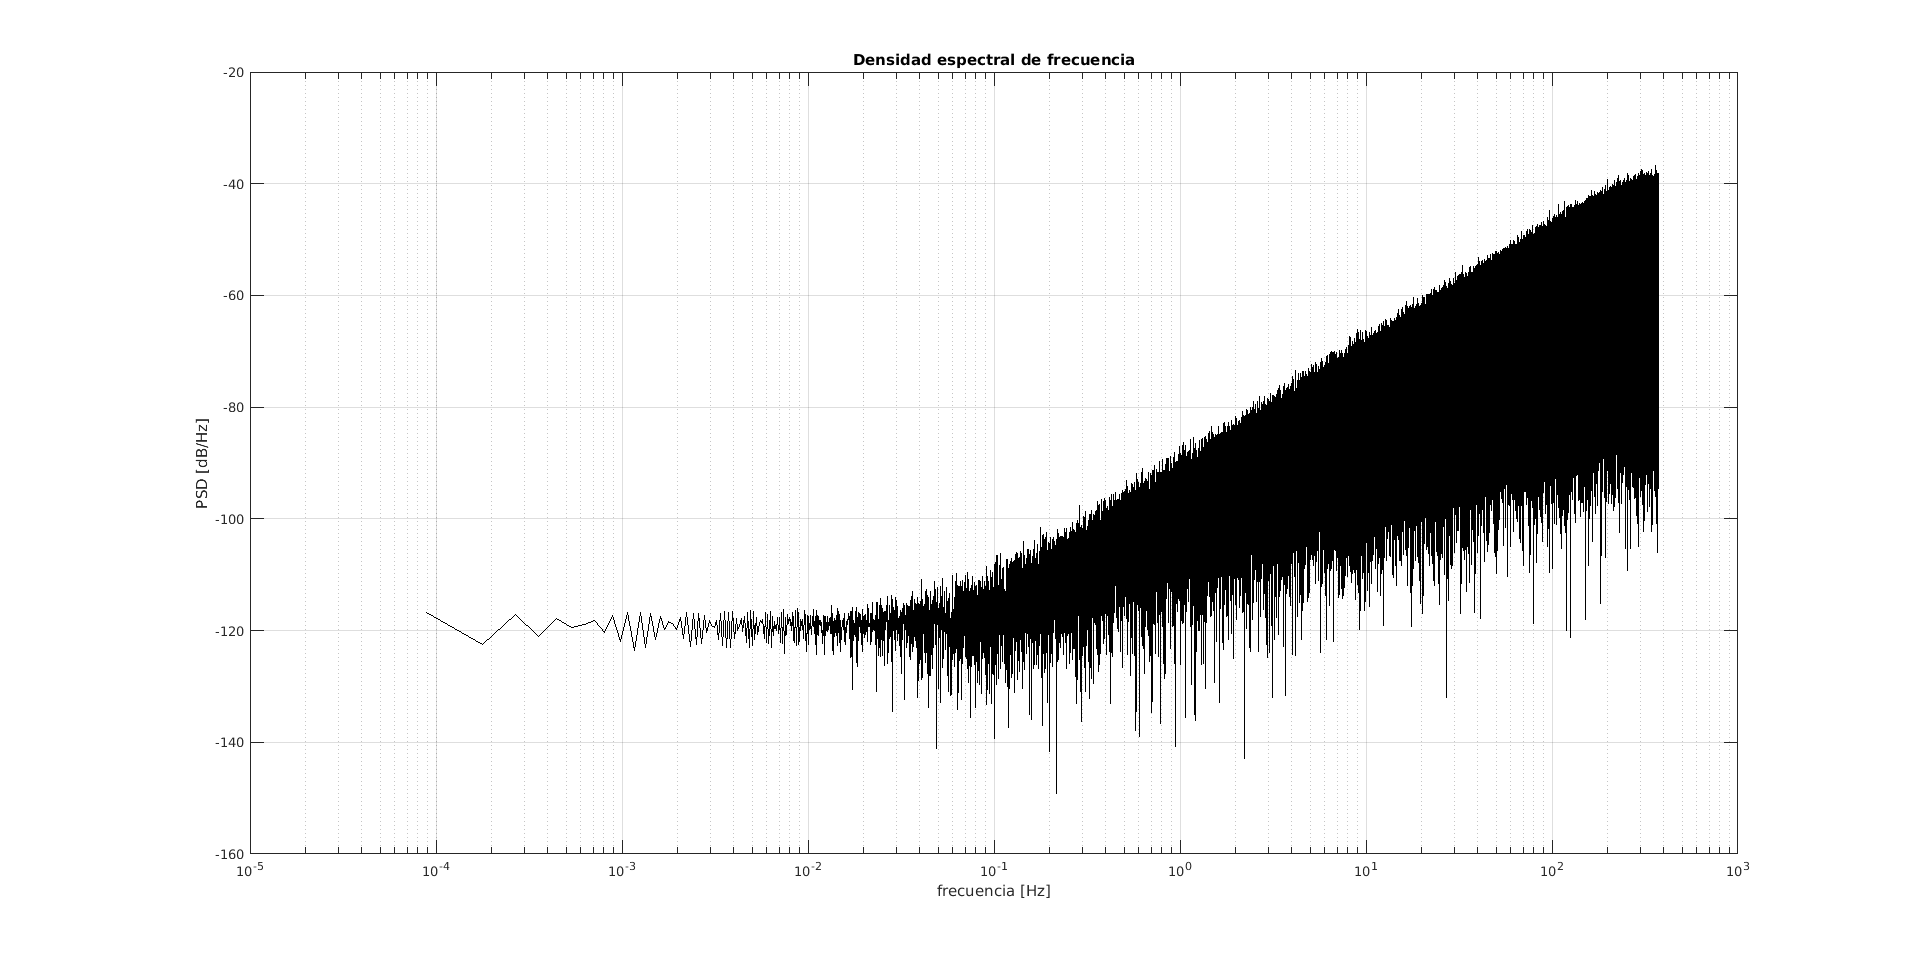
\includegraphics[width=8cm]{Figuras/PSDQuantizationNoise.png}
        \caption{PSD: quantization noise}
        \label{fig:}
    \end{subfigure}%
    \begin{subfigure}[t]{0.5\textwidth}
        \centering
        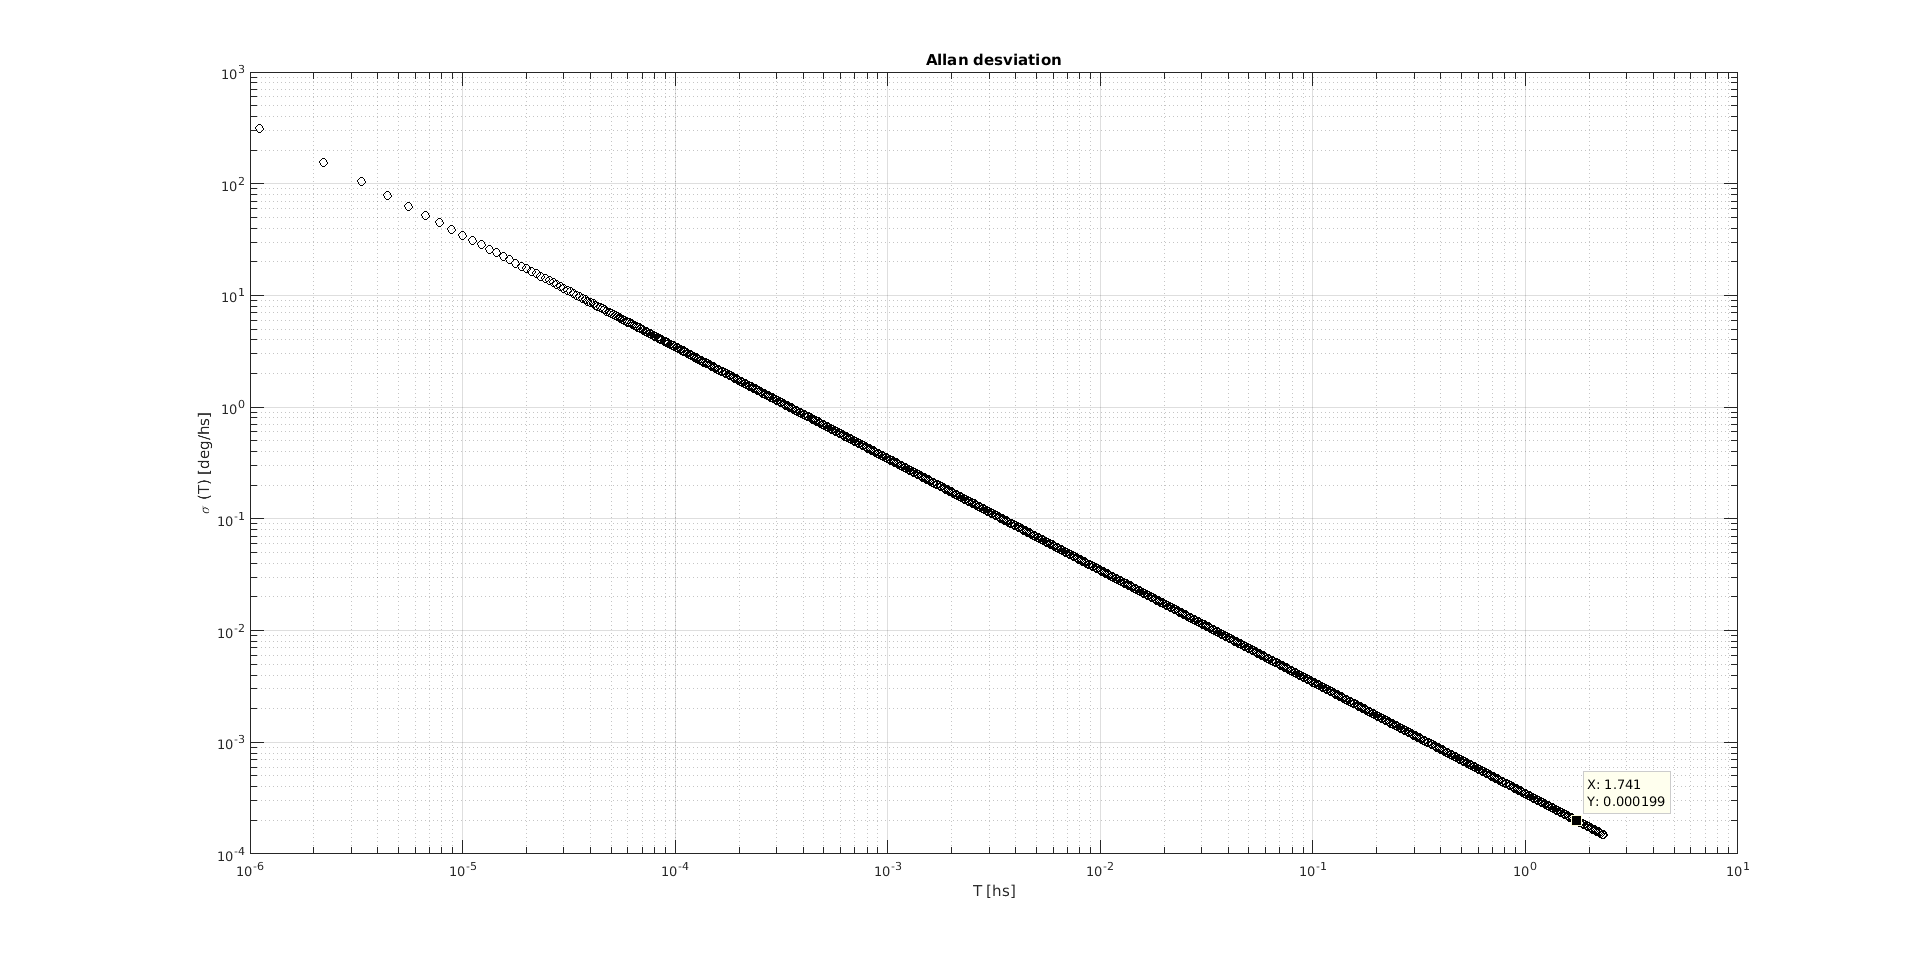
\includegraphics[width=8cm]{Figuras/AllanQuantizationNoise.png}
        \caption{Allan desviation: quantization noise}
        \label{fig:}
    \end{subfigure}%
    ~ 
    \caption{Simulación quantization noise}
    \label{fig:simulacionquantizationNoise}
\end{figure*}
\begin{figure*}[t!]
    \centering
    \begin{subfigure}[t]{0.5\textwidth}
        \centering
        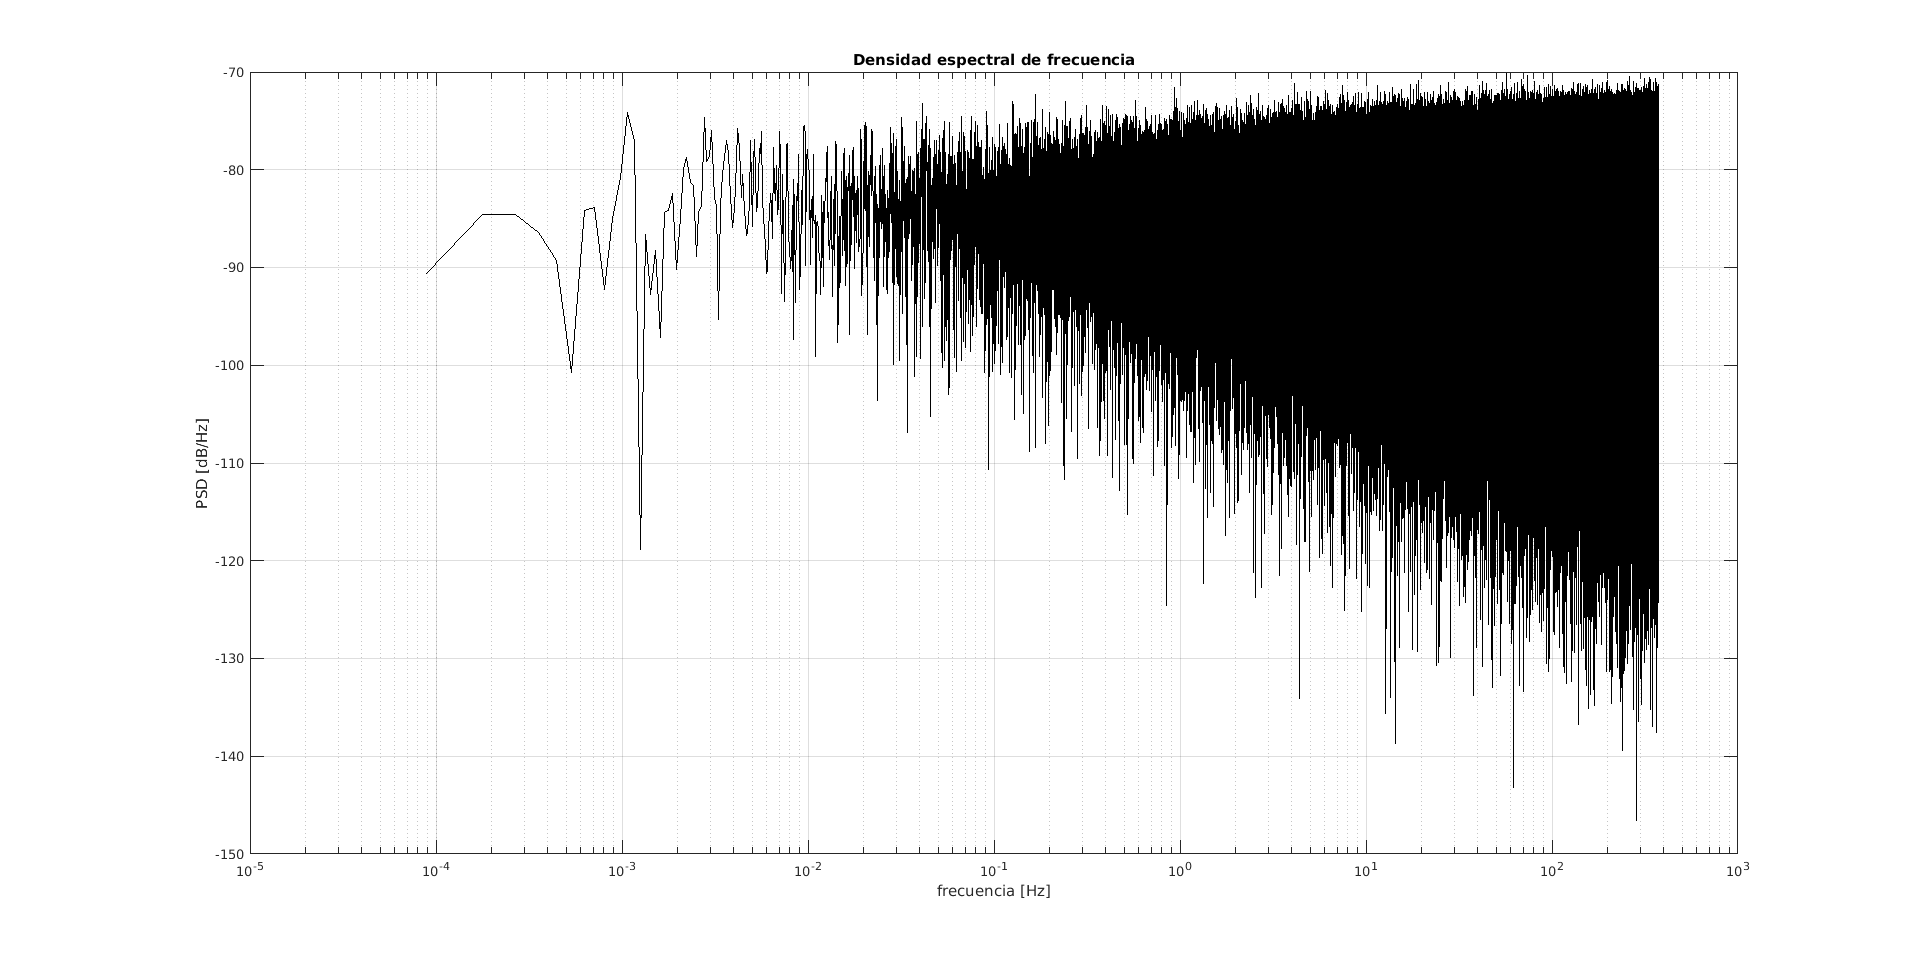
\includegraphics[width=8cm]{Figuras/PSDARW.png}
        \caption{PSD: angle random walk}
        \label{fig:}
    \end{subfigure}%
    \begin{subfigure}[t]{0.5\textwidth}
        \centering
        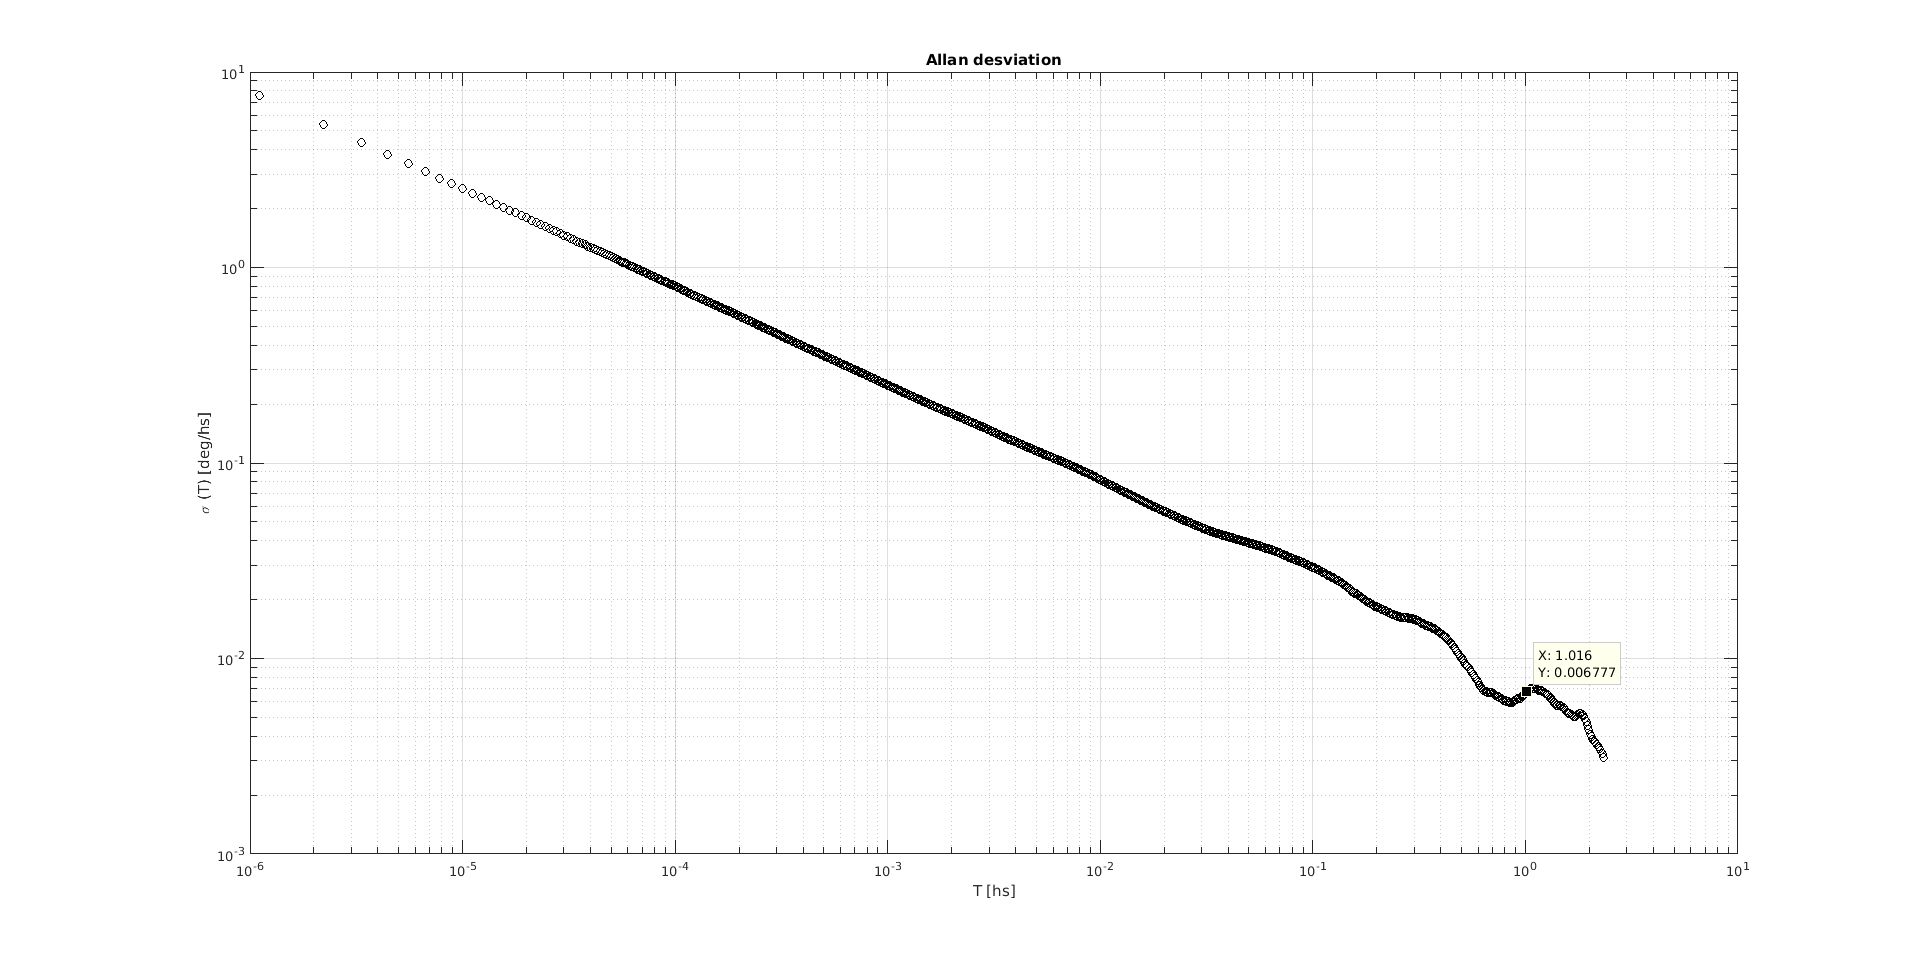
\includegraphics[width=8cm]{Figuras/AllanARW.png}
        \caption{Allan desviation: angle random walk}
        \label{fig:}
    \end{subfigure}%
    ~ 
    \caption{Simulación angle random walk}
    \label{fig:simulacionARW}
\end{figure*}
\begin{figure*}[t!]
    \centering
    \begin{subfigure}[t]{0.5\textwidth}
        \centering
        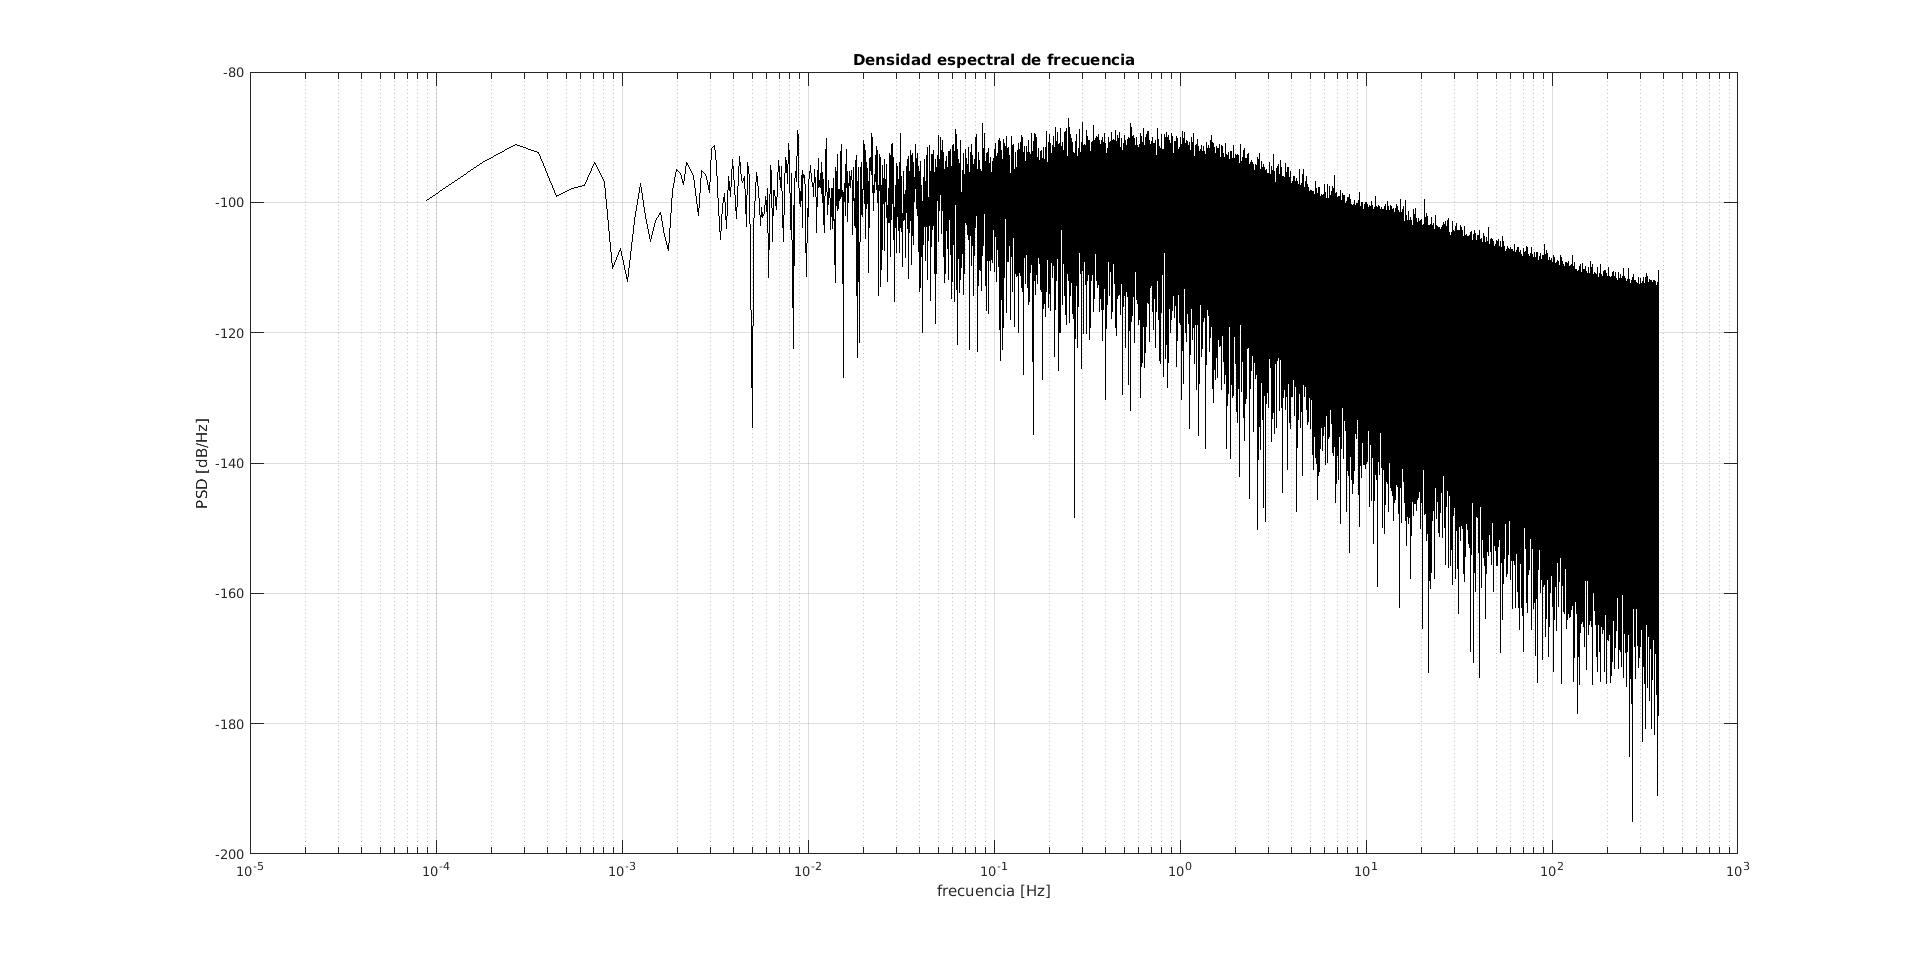
\includegraphics[width=8cm]{Figuras/PSDBI.png}
        \caption{PSD: bias instability}
        \label{fig:}
    \end{subfigure}%
    \begin{subfigure}[t]{0.5\textwidth}
        \centering
        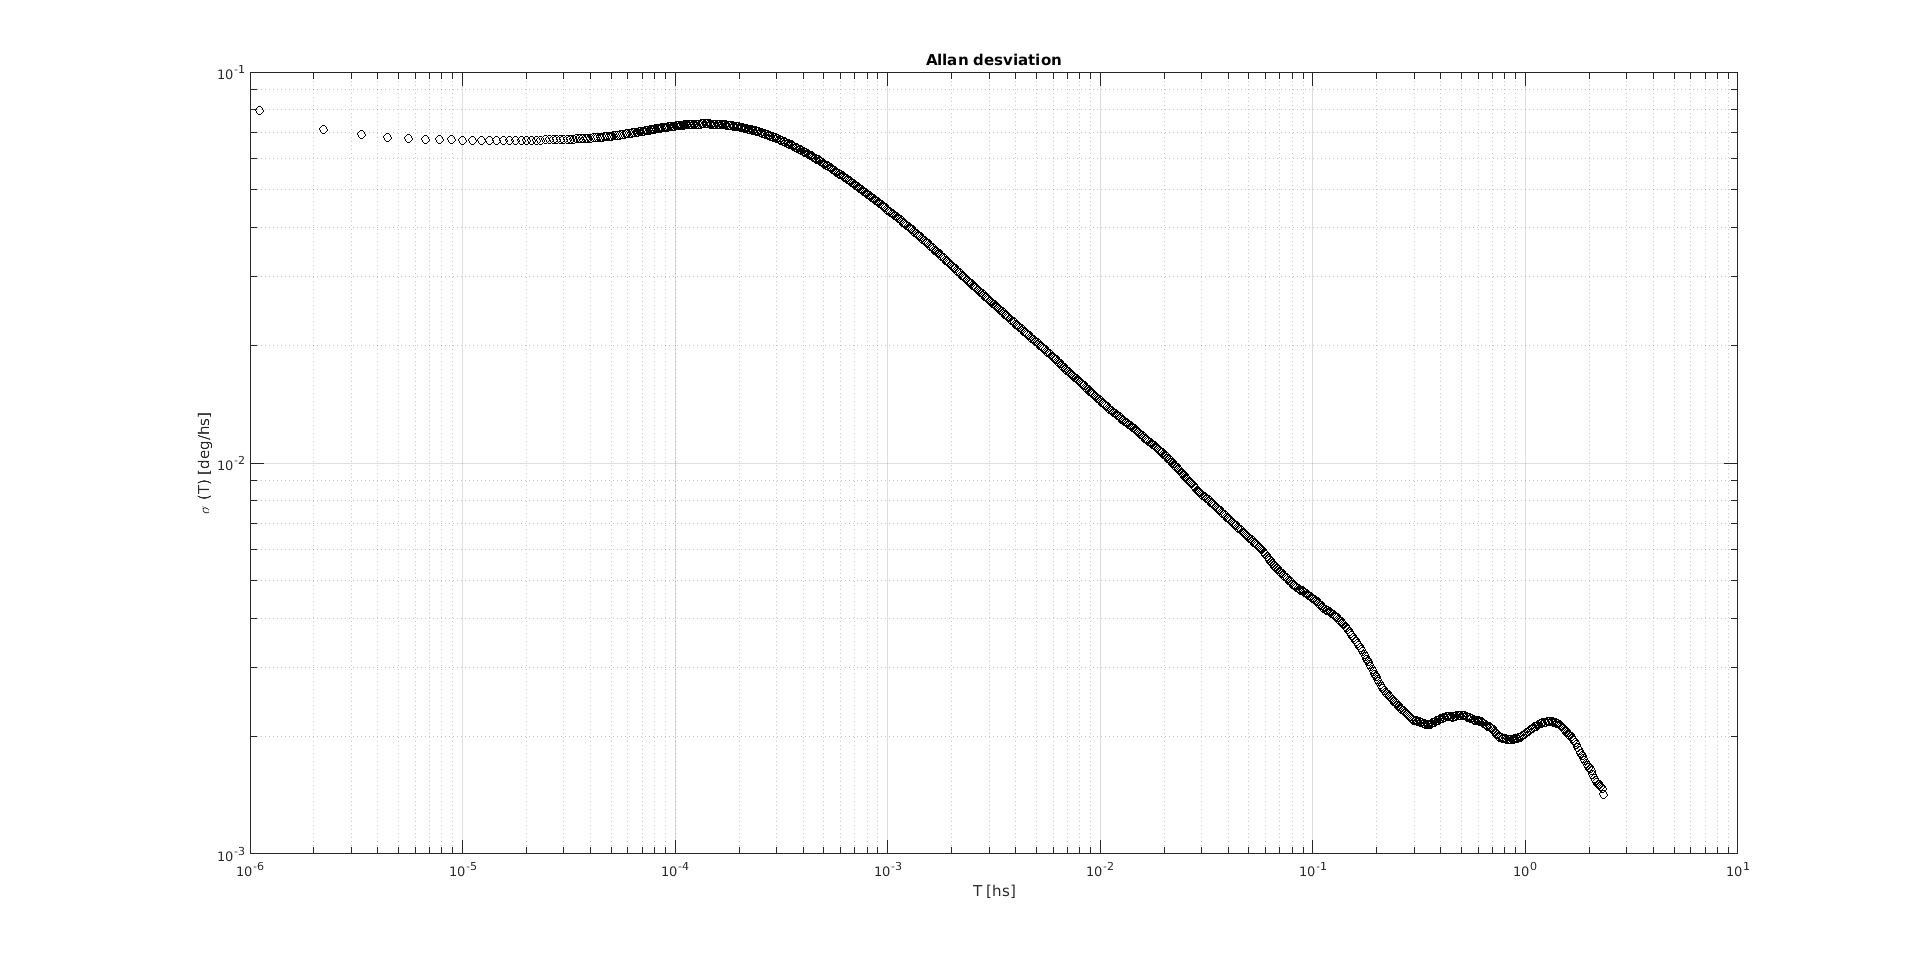
\includegraphics[width=8cm]{Figuras/AllanBI.png}
        \caption{Allan desviation: bias instability}
        \label{fig:}
    \end{subfigure}%
    ~ 
    \caption{Simulación bias instability}
    \label{fig:simulacionBI}
\end{figure*}
\begin{figure*}[t!]
    \centering
    \begin{subfigure}[t]{0.5\textwidth}
        \centering
        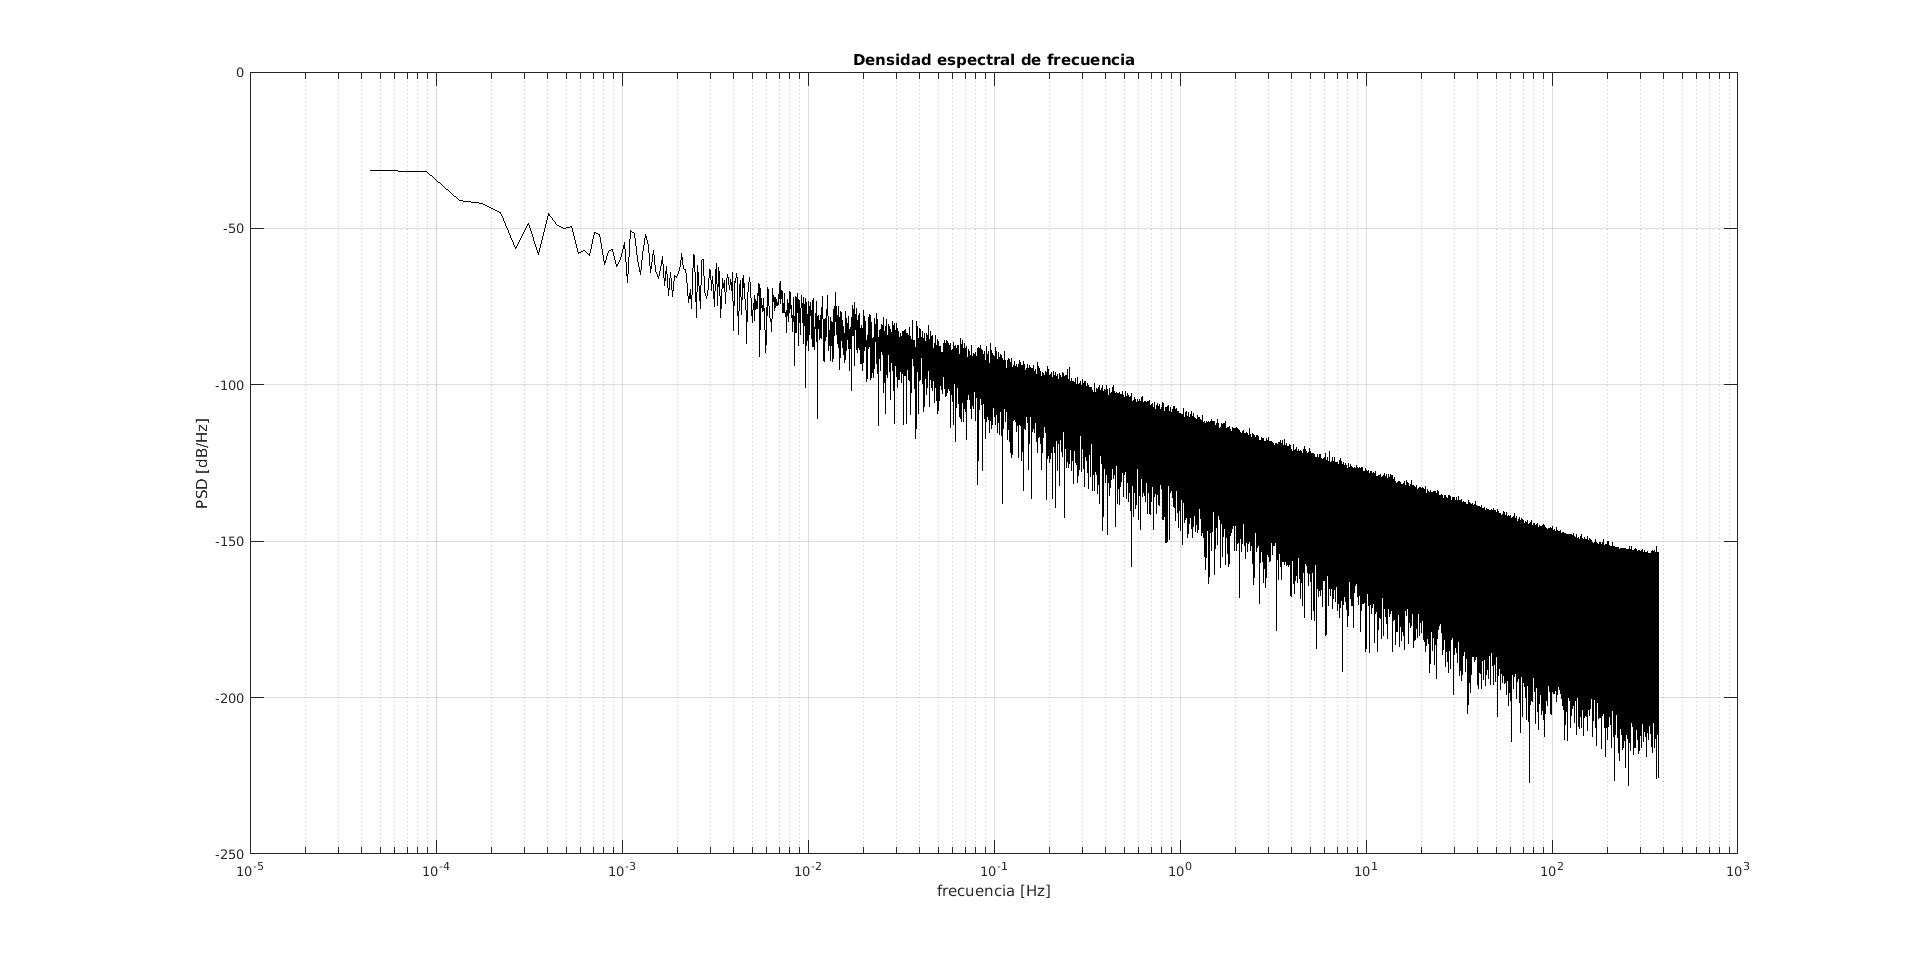
\includegraphics[width=8cm]{Figuras/PSDRRW.png}
        \caption{PSD: rate random walk}
        \label{fig:}
    \end{subfigure}%
    \begin{subfigure}[t]{0.5\textwidth}
        \centering
        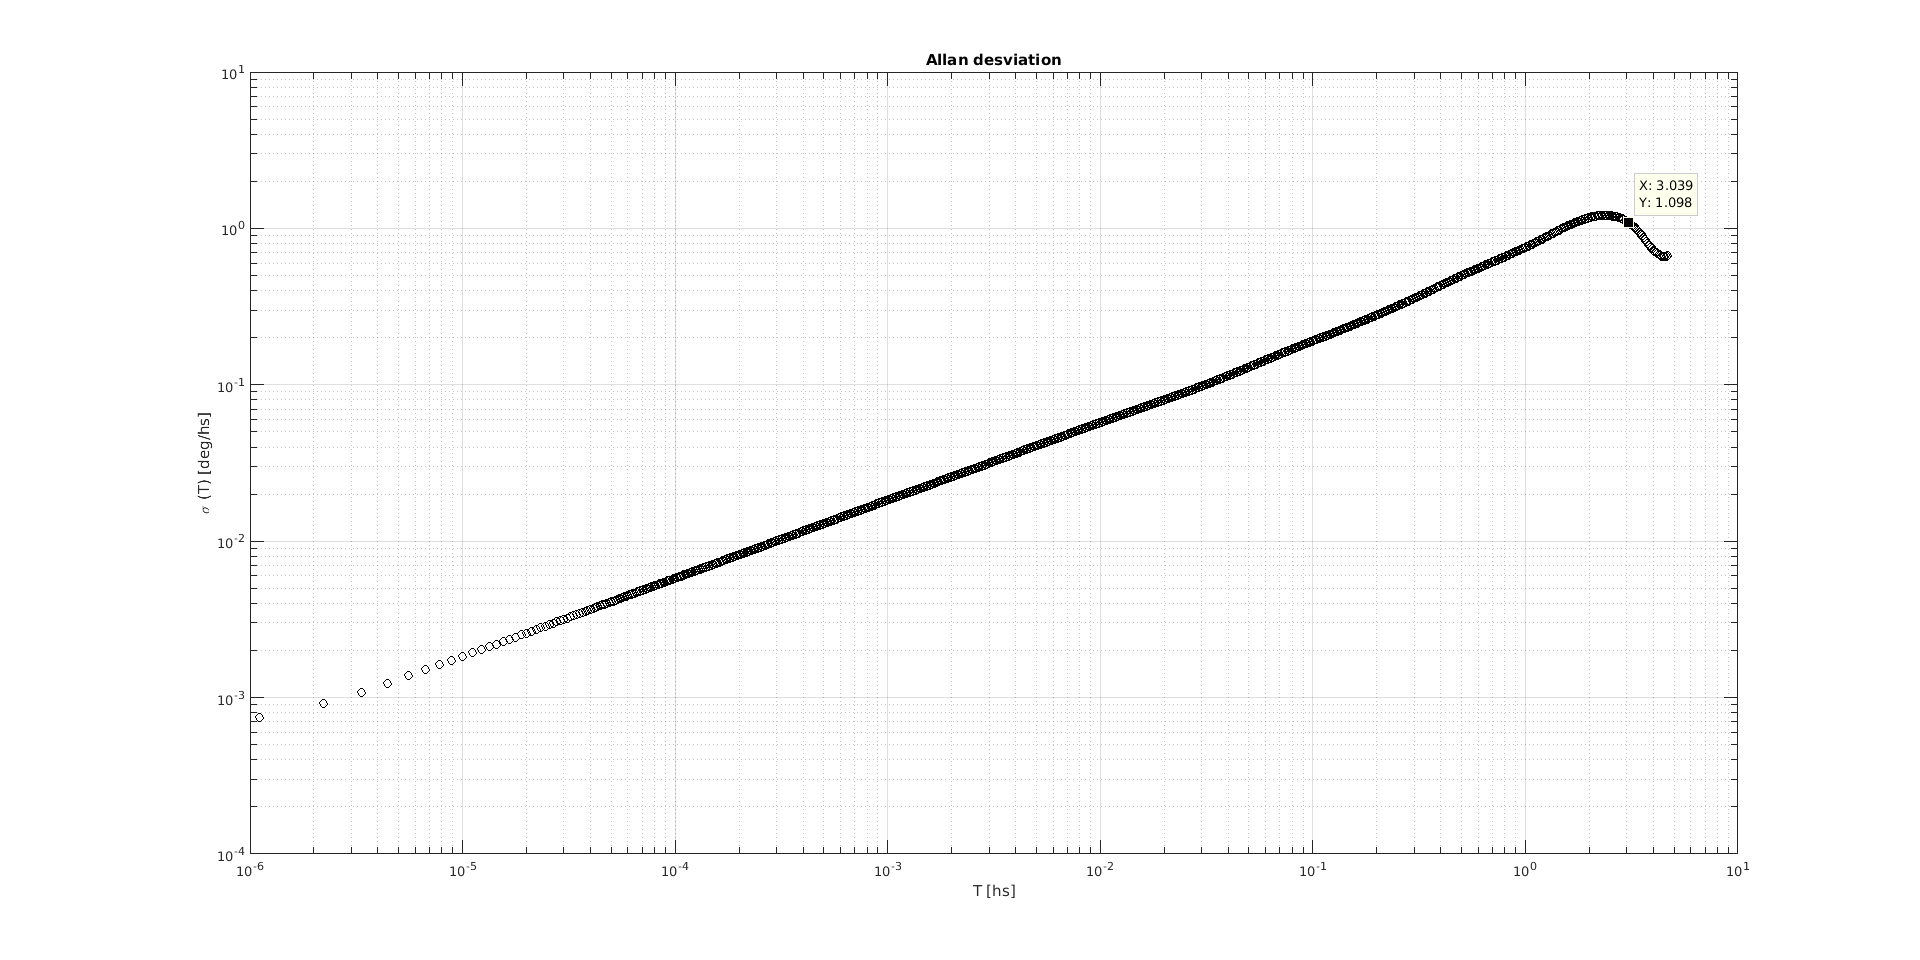
\includegraphics[width=8cm]{Figuras/AllanRRW.png}
        \caption{Allan desviation: rate random walk}
        \label{fig:}
    \end{subfigure}%
    ~ 
    \caption{Simulación rate random walk}
    \label{fig:simulacionRRW}
\end{figure*}
\begin{figure*}[t!]
    \centering
    \begin{subfigure}[t]{0.5\textwidth}
        \centering
        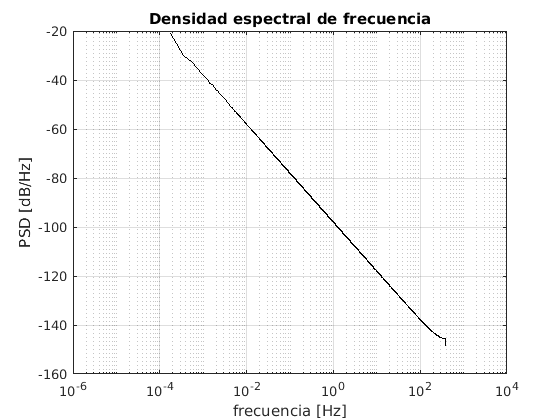
\includegraphics[width=8cm]{Figuras/PSDRR.png}
        \caption{PSD: drift rate ramp}
        \label{fig:}
    \end{subfigure}%
    \begin{subfigure}[t]{0.5\textwidth}
        \centering
        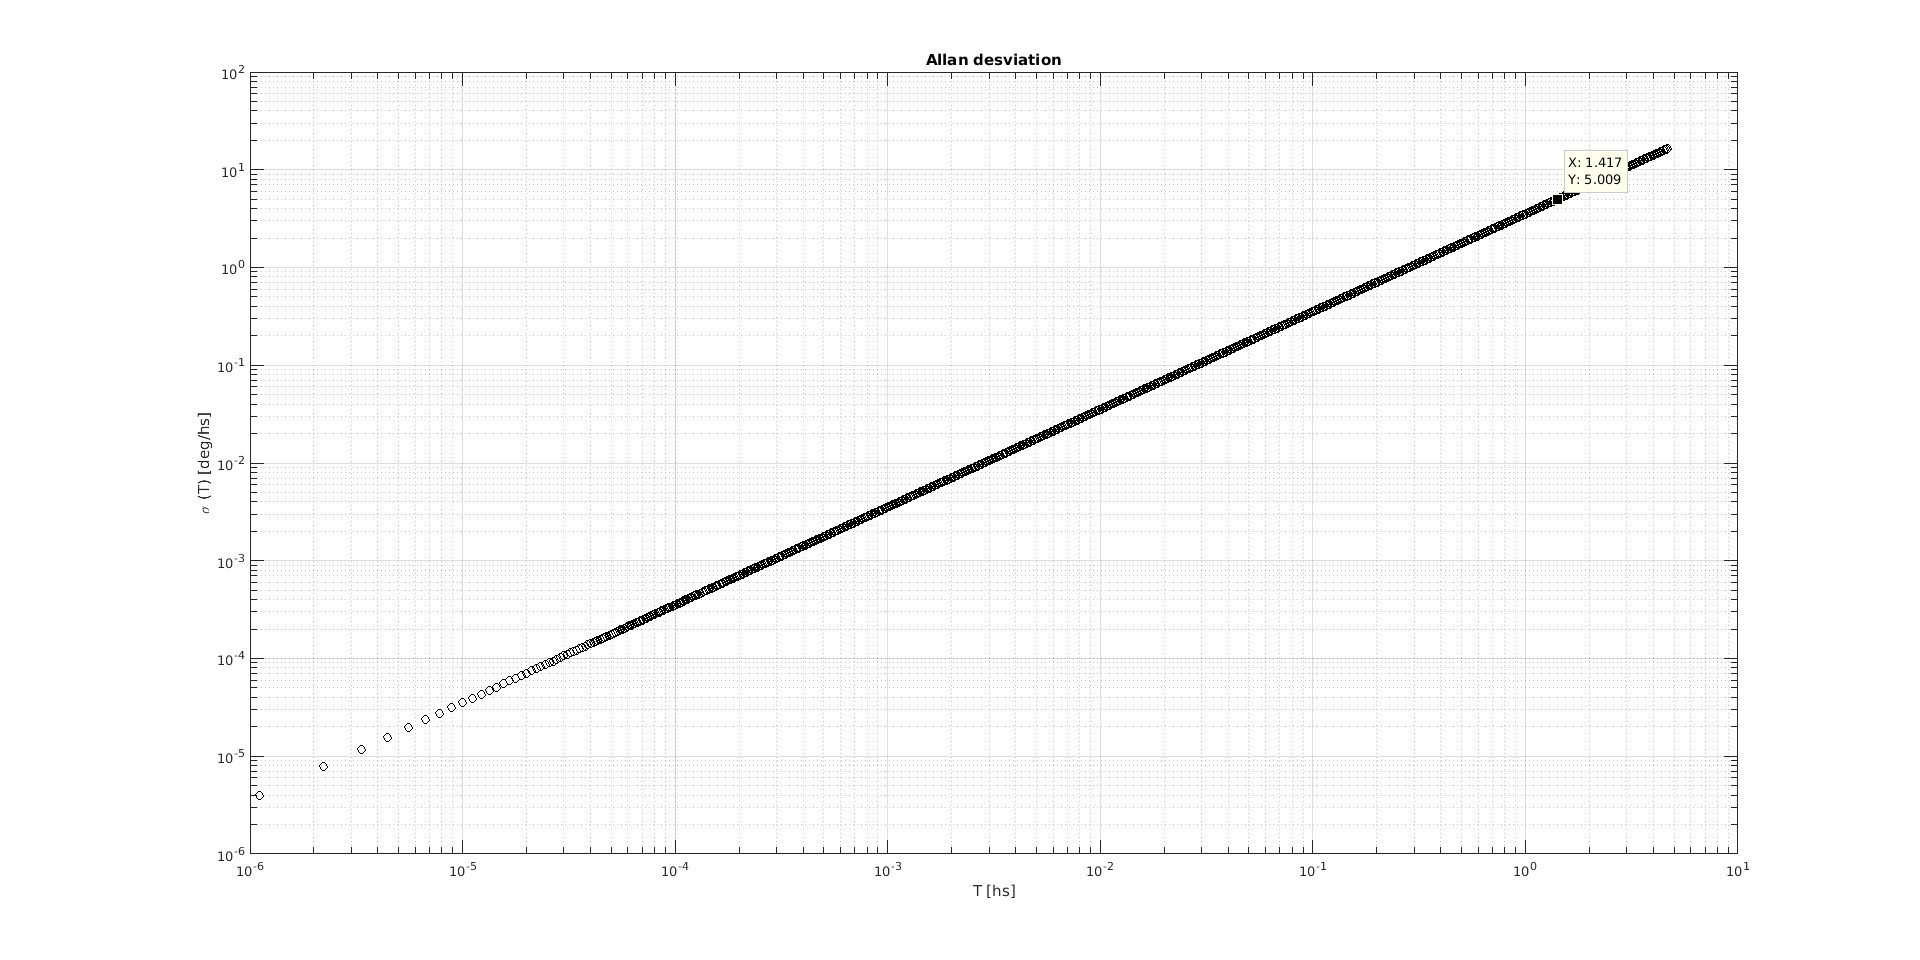
\includegraphics[width=8cm]{Figuras/AllanRR.png}
        \caption{Allan desviation: drift rate ramp}
        \label{fig:}
    \end{subfigure}%
    ~ 
    \caption{Simulación drift rate ramp}
    \label{fig:simulacionRR}
\end{figure*}
\begin{figure*}[t!]
    \centering
    \begin{subfigure}[t]{0.5\textwidth}
        \centering
        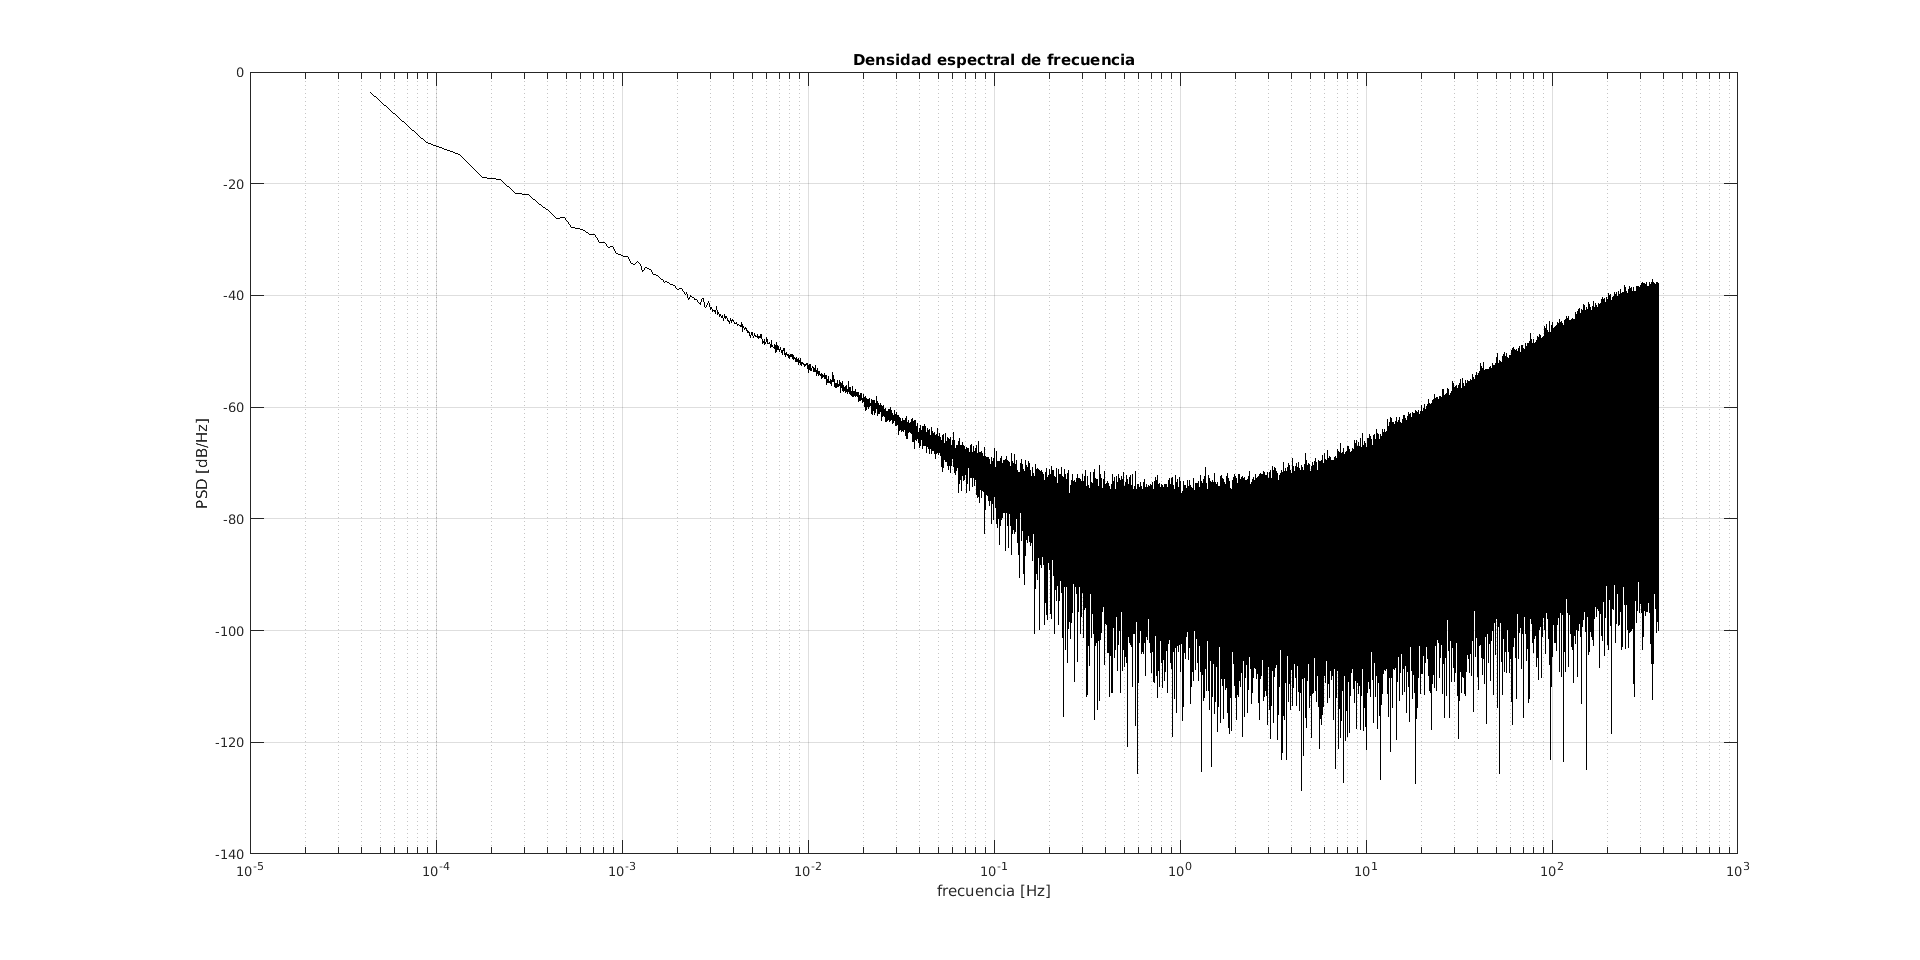
\includegraphics[width=8cm]{Figuras/PSDRuidosTodos.png}
        \caption{PSD: contribución de todas las componentes}
        \label{fig:}
    \end{subfigure}%
    \begin{subfigure}[t]{0.5\textwidth}
        \centering
        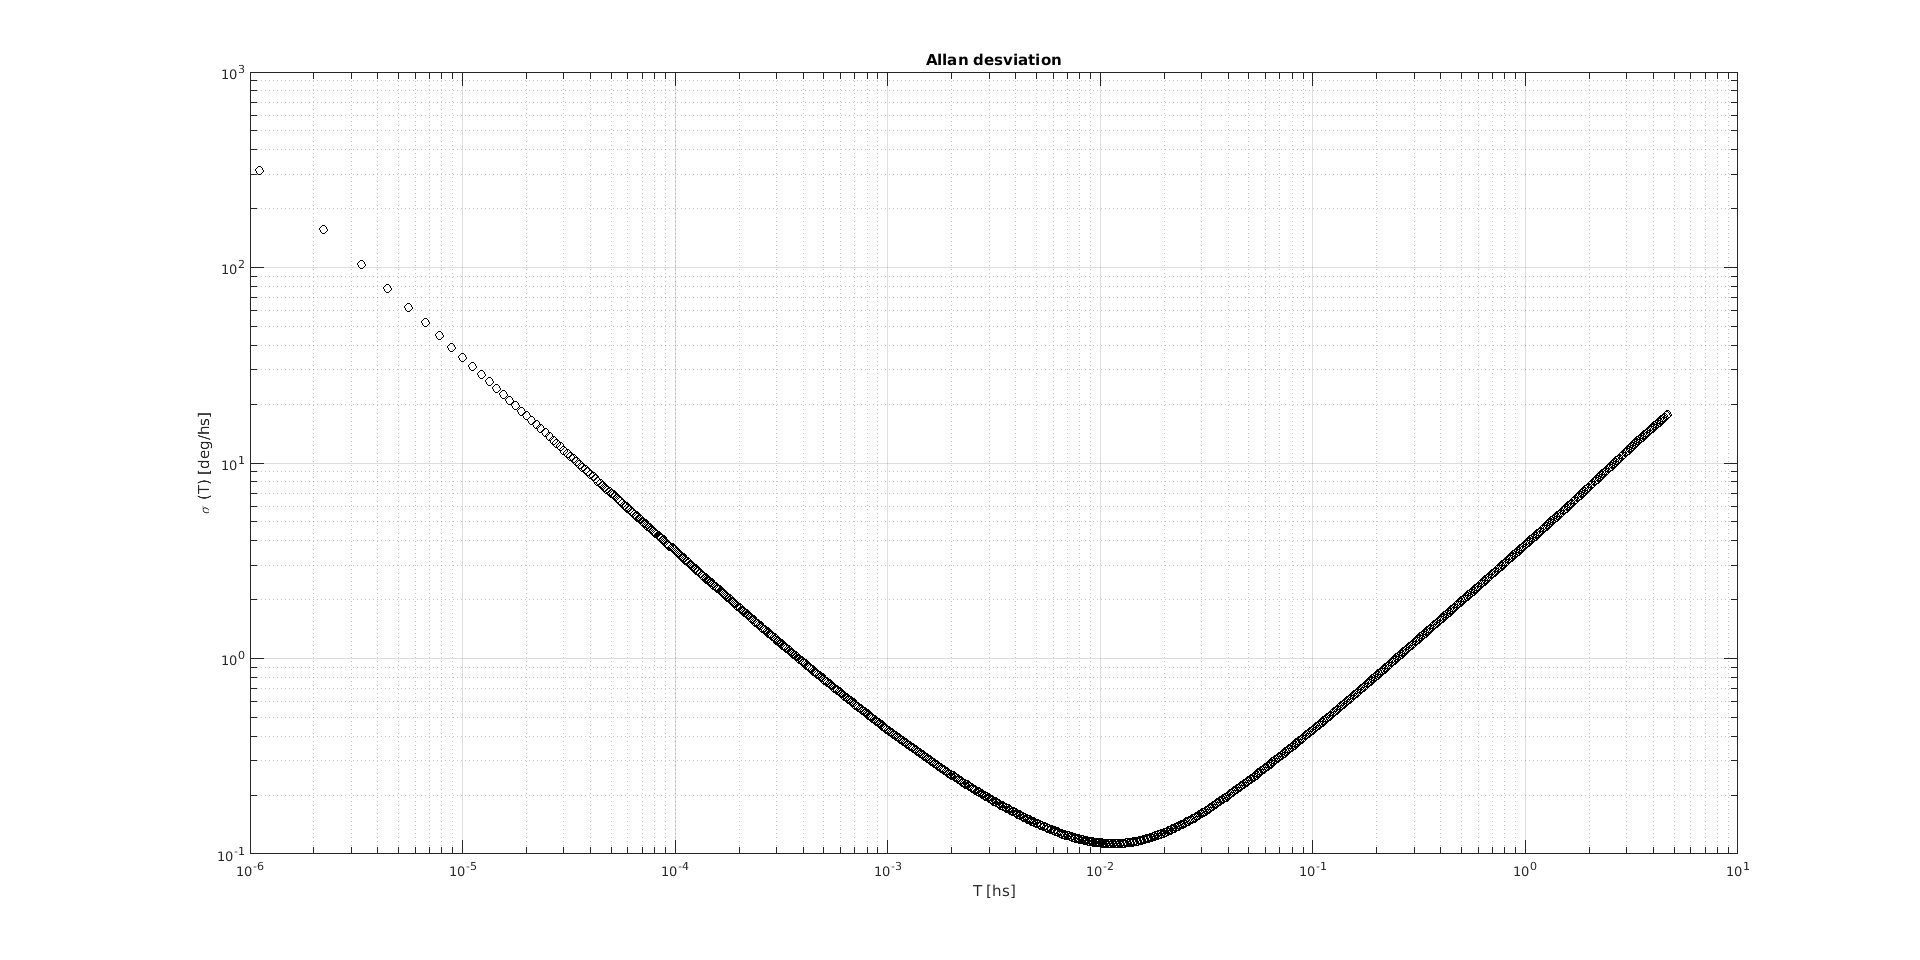
\includegraphics[width=8cm]{Figuras/AllanRuidosTodos.png}
        \caption{Allan desviation: contribución de todas las componentes}
        \label{fig:}
    \end{subfigure}%
    ~ 
    \caption{Simulación de la contribución de todas las componentes}
    \label{fig:simulacionRuidosTodos}
\end{figure*}
\begin{figure}[h!]
\centering
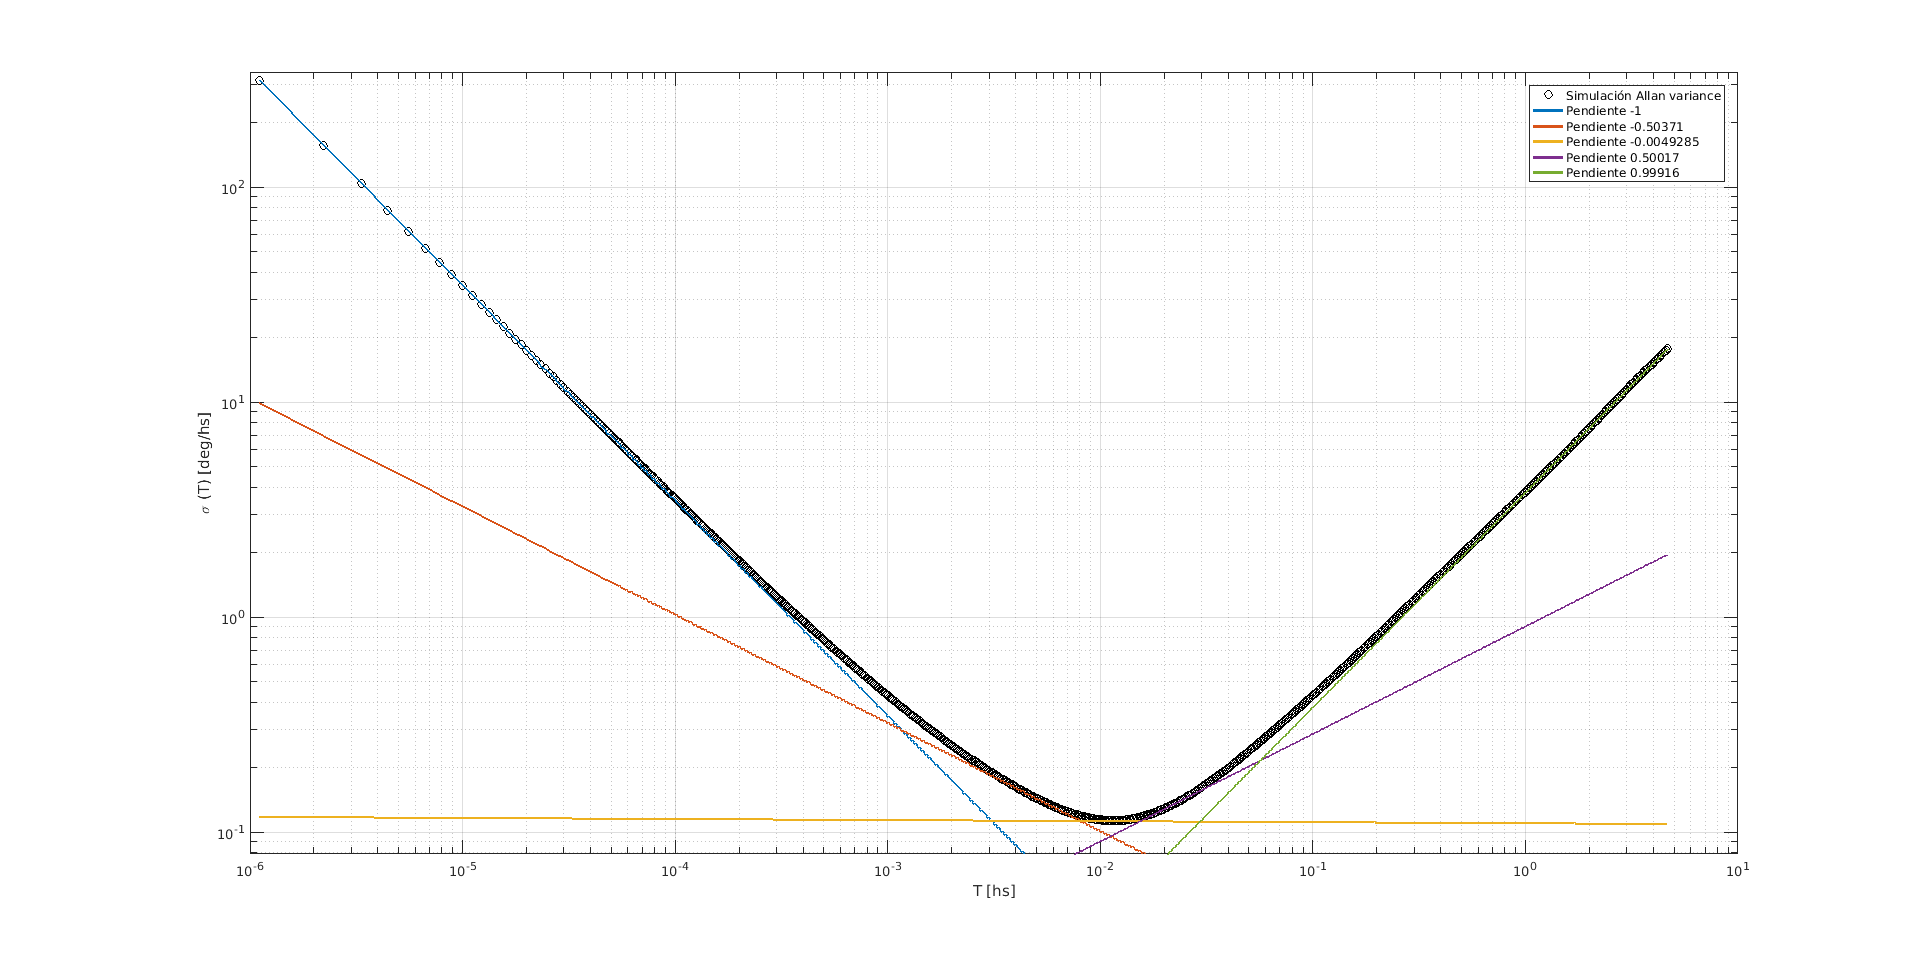
\includegraphics[width=8cm]{Figuras/AllanRuidosTodosConRectas.png}
\caption{Allan desviation de la contribución de todas las componentes junto con las rectas características.}
\label{fig:simulacionRuidosTodosRectas}
\end{figure}
\par En la Fig. Nº\ref{fig:simulacionRuidosTodos} se muestra el aporte de todas las componentes; es decir, la suma de todos los ruidos anteriormente simulados. En la Fig. Nº\ref{fig:simulacionRuidosTodosRectas} se añadieron las rectas con las pendientes características más cercanas a los valores teóricos. Para esto, se calculó cada pendiente entre dos puntos consecutivos. 
\par Las simulaciones de cada una de las componentes permiten verificar lo que predice cada uno de los resultados teóricos. Se puede verificar el valor del coeficiente utilizado para cada uno de los valores de $T$ correspondientes  (como así también la relación indicada para el caso de bias instability). Sin embargo, al tratar con todas las componentes en simultáneo se nota como algunas acaban predominando más que otras. Por ello es útil observar la PSD. En la PSD de la Fig. Nº\ref{fig:simulacionRuidosTodos} se aprecia que los ruidos mejor distinguibles son del tipo drift rate rap, angle random walk y quantization noise. La Fig. Nº\ref{fig:simulacionRuidosTodosRectas} expone este resultado con una mejor mayor aproximación  a lo largo del tiempo promedio $T$ de las rectas características, principalmente para ``el'' quantization noise y ``el'' drift rate ramp.
\section{ANÁLISIS DE DATOS DE UN GIRÓSCOPO}
Se cuenta con lecturas del giróscopo I3DM-GX3-35 de tecnología MEMS. Estas lecturas se realizaron con el dispositivo adquiriendo datos en reposo; es decir, sin movimiento. Se asume que los datos se encuentran en unidades de $rad/s$. Dado que el código construido se concibió para operar en $deg/s$, los datos se multiplican por un factor de $180/\pi$.
\\En las figuras Nº\ref{fig:lecturasEjex}, Nº\ref{fig:lecturasEjey} y Nº\ref{fig:lecturasEjez} se muestran las PSD y ``el'' Allan desviation para las lecturas de cada eje (\textit{x}, \textit{y} y \textit{z}) y en las figuras Nº\ref{fig:lecturaEjexRectas}, Nº\ref{fig:lecturaEjeyRectas} y Nº\ref{fig:lecturaEjezRectas} se muestra el Allan desviation junto con las rectas características. 
\\ De acuerdo a las gráficas de PSD, las componentes que mejor se exhiben son principalmente angle random walk y en menor medida, bias instability. Claramente esto se verifica en cada uno de los gráficos de Allan desviation. En las figuras donde se añaden las rectas, se aprecia como las rectas con pendientes cercanas a $-1/2$ y $0$ se \textit{unen} a los puntos del gráfico en las regiones que son de esperar, mientras que para las restantes pendientes las rectas se adhieren a puntos que carecen de sentido. 
\\ De las figuras Nº\ref{fig:lecturaEjexRectas}, Nº\ref{fig:lecturaEjeyRectas} y Nº\ref{fig:lecturaEjezRectas} se puede inferir el valor de algunos de los coeficientes de las componentes que se distinguen; es decir, $Q$ y $B$ para los tres ejes, y $Q_z$ solo para el eje x. Los valores inferidos se muestran en la tabla Nº\ref{tabla:valoresCoeficientesEjes}.
%q
%Q
\begin{figure*}[t!]
    \centering
    \begin{subfigure}[t]{0.5\textwidth}
        \centering
        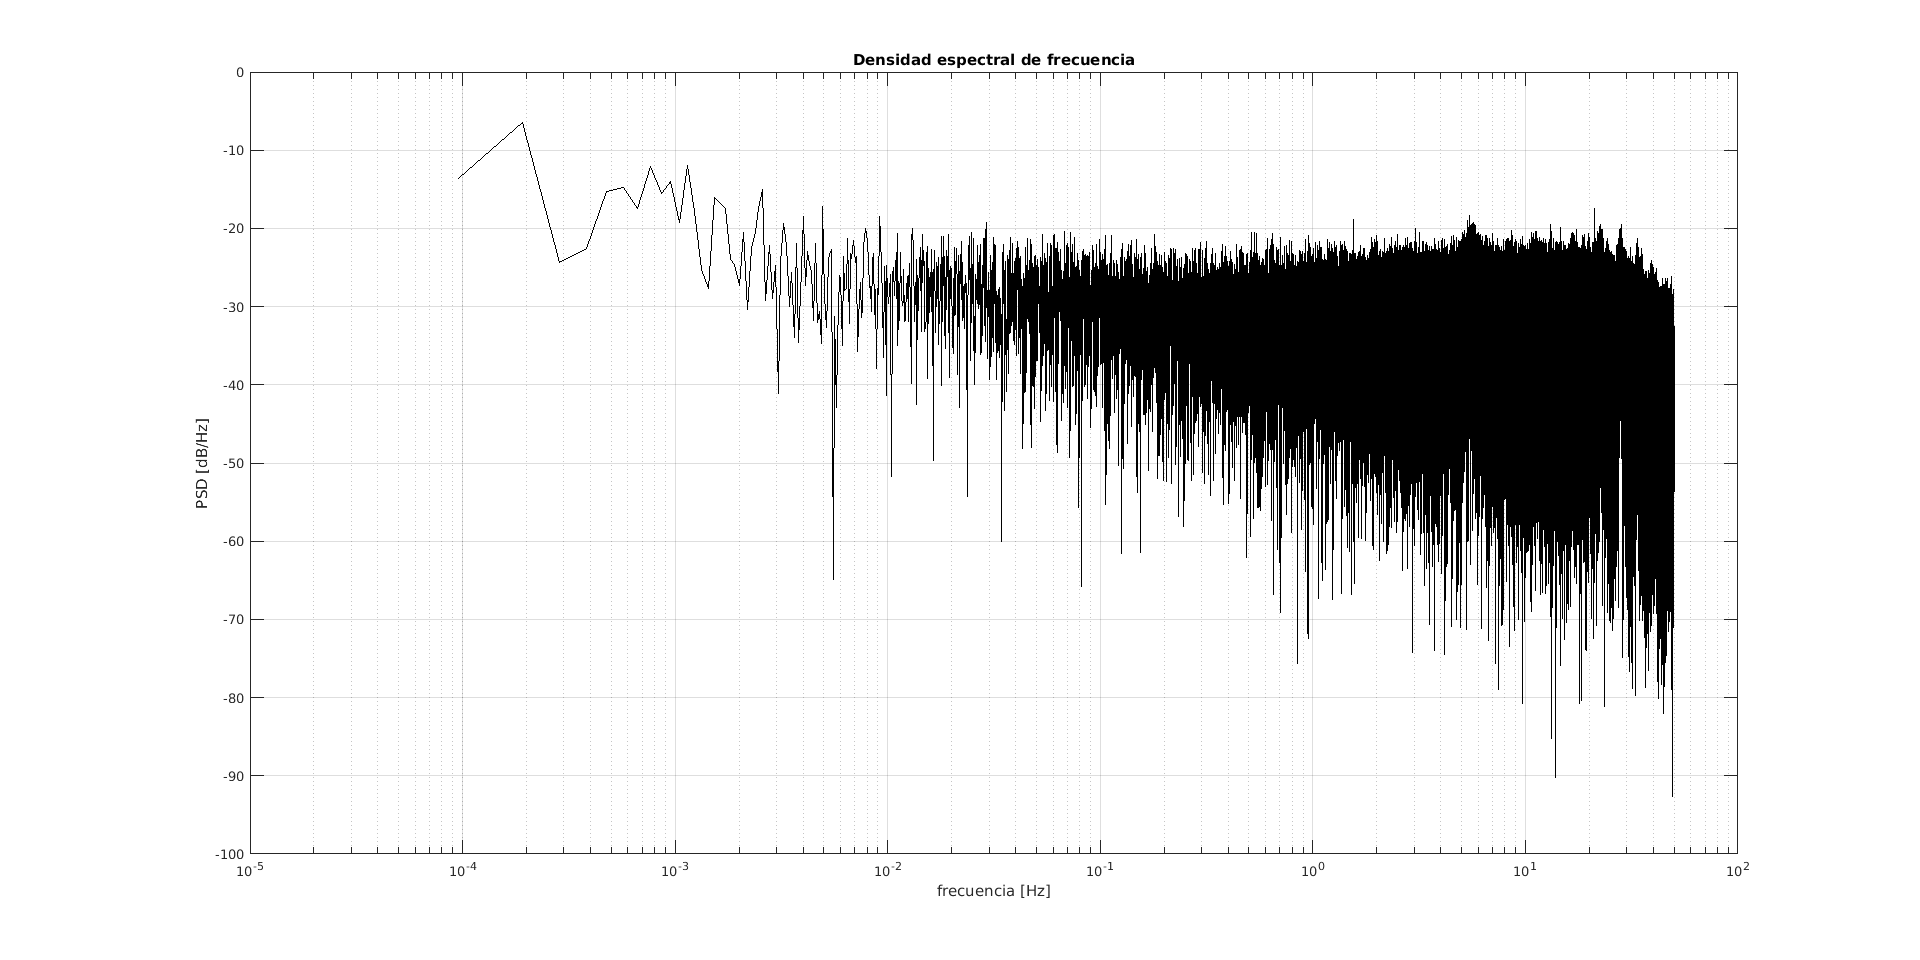
\includegraphics[width=8cm]{Figuras/PSDGyrox.png}
        \caption{PSD: lecturas eje x}
        \label{fig:}
    \end{subfigure}%
    \begin{subfigure}[t]{0.5\textwidth}
        \centering
        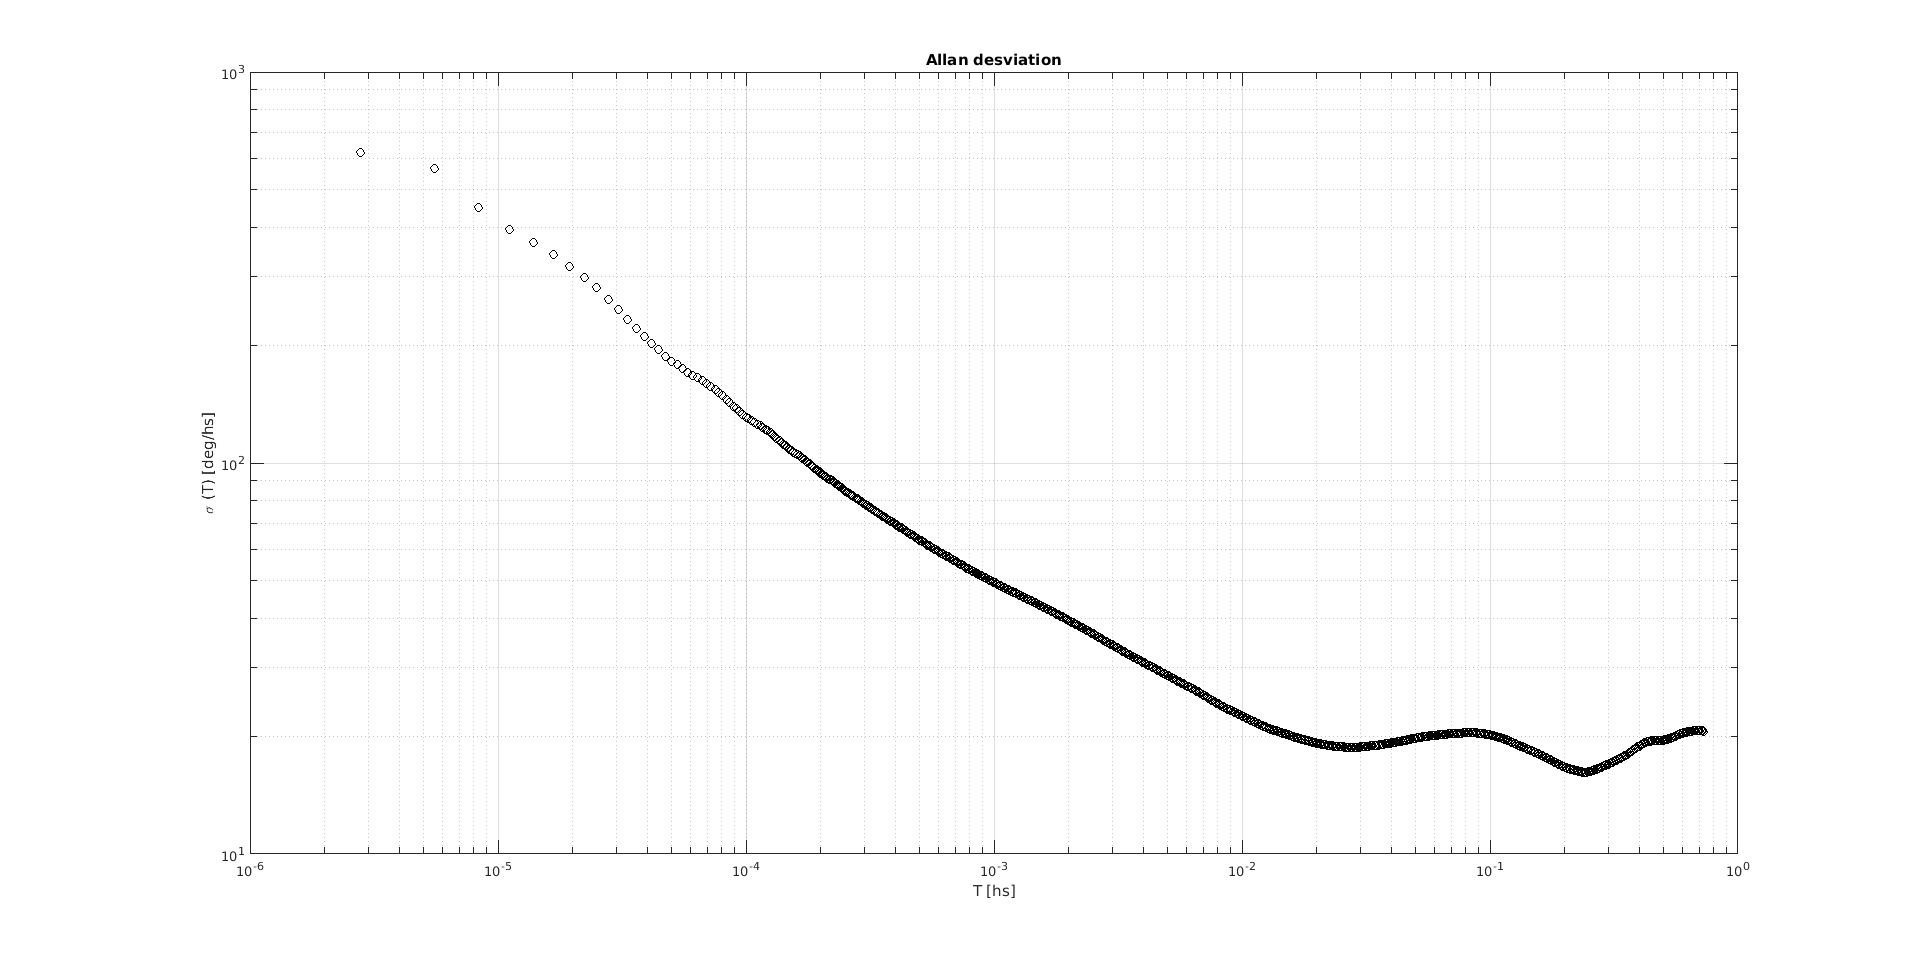
\includegraphics[width=8cm]{Figuras/AllanGyrox.png}
        \caption{Allan desviation: lecturas eje x}
        \label{fig:}
    \end{subfigure}%
    ~ 
    \caption{Lectura del eje x}
    \label{fig:lecturasEjex}
\end{figure*}
\begin{figure}[h!]
\centering
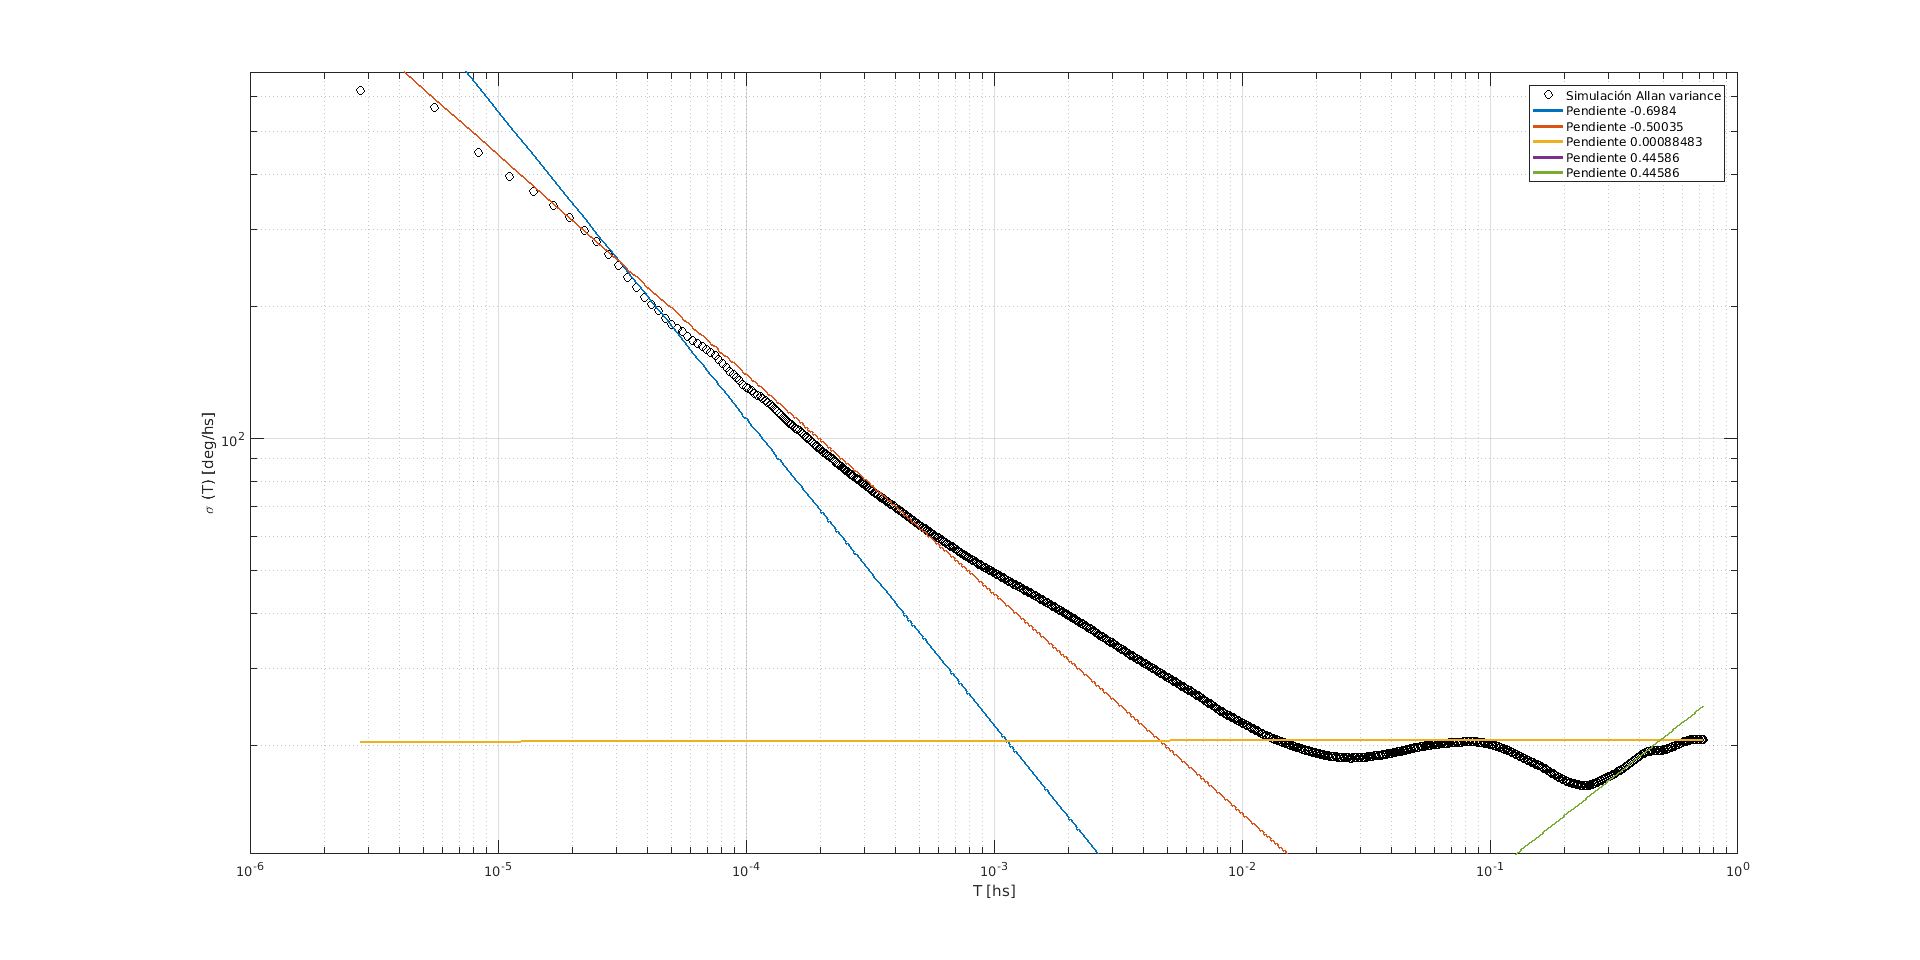
\includegraphics[width=8cm]{Figuras/AllanGyroxRectas.png}
\caption{Allan desviation del eje x junto con las rectas características}
\label{fig:lecturaEjexRectas}
\end{figure}
\begin{figure*}[t!]
    \centering
    \begin{subfigure}[t]{0.5\textwidth}
        \centering
        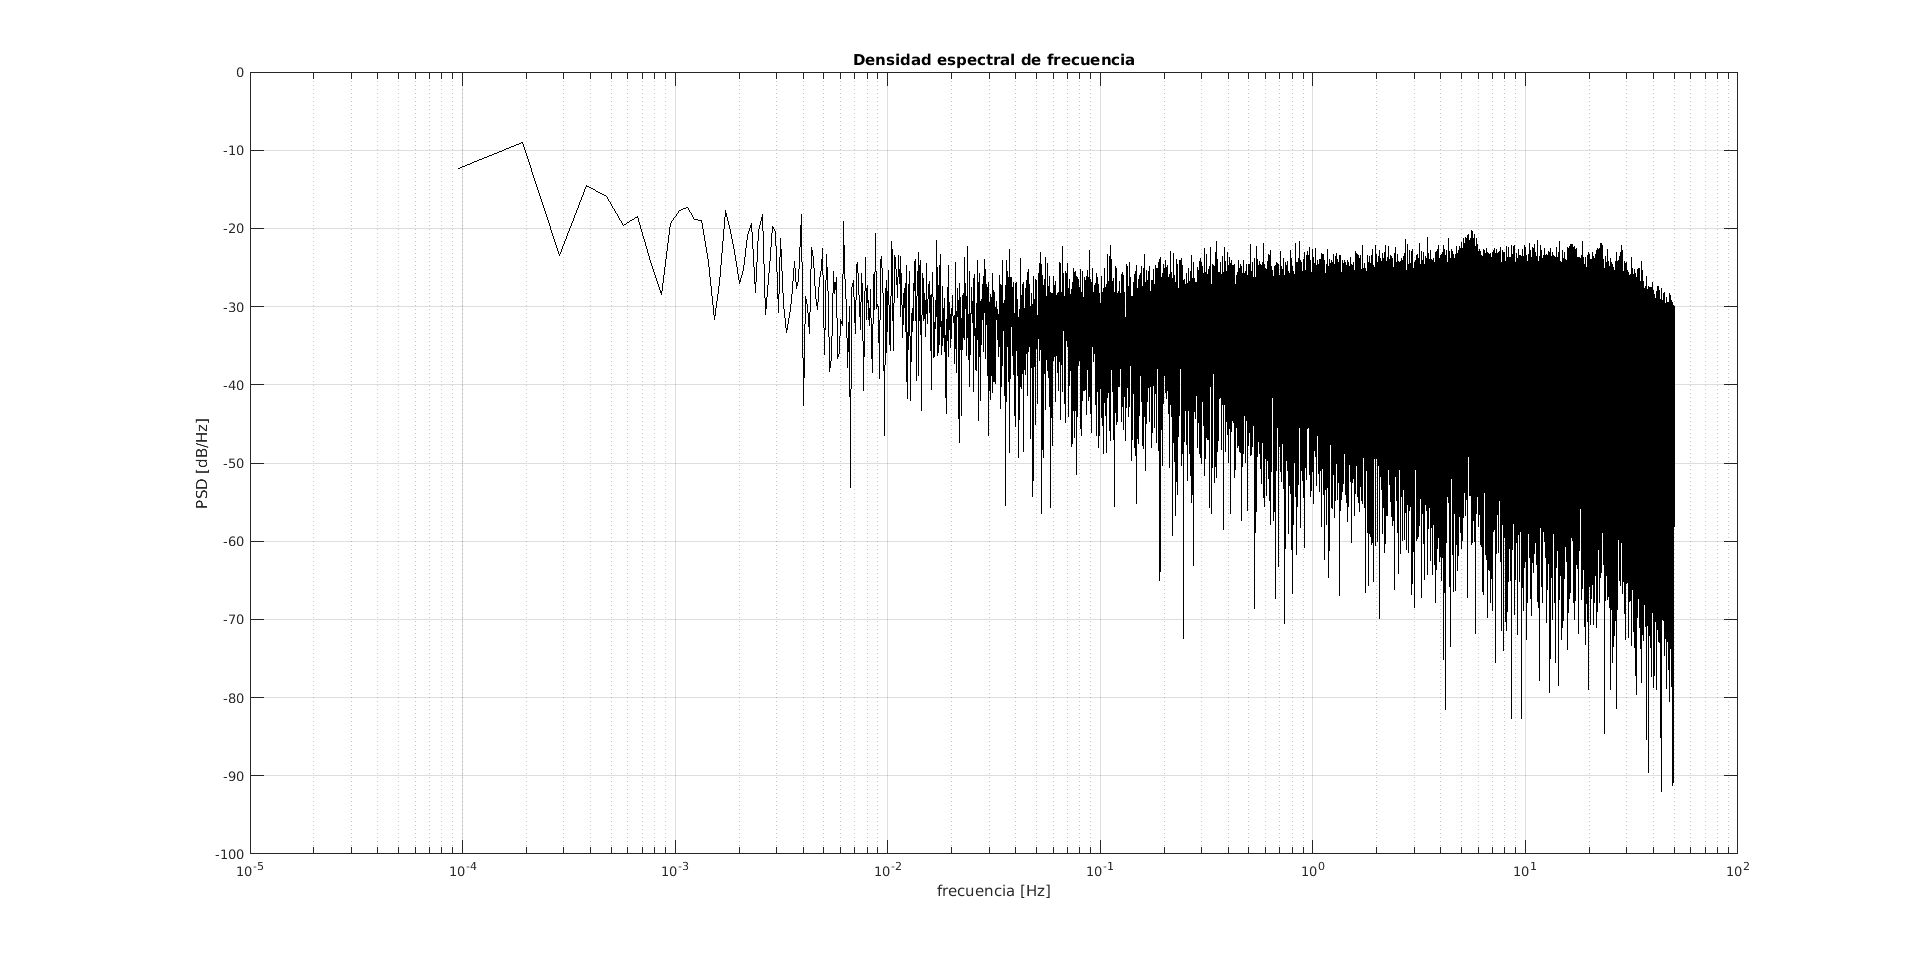
\includegraphics[width=8cm]{Figuras/PSDGyroy.png}
        \caption{PSD: lecturas eje y}
        \label{fig:}
    \end{subfigure}%
    \begin{subfigure}[t]{0.5\textwidth}
        \centering
        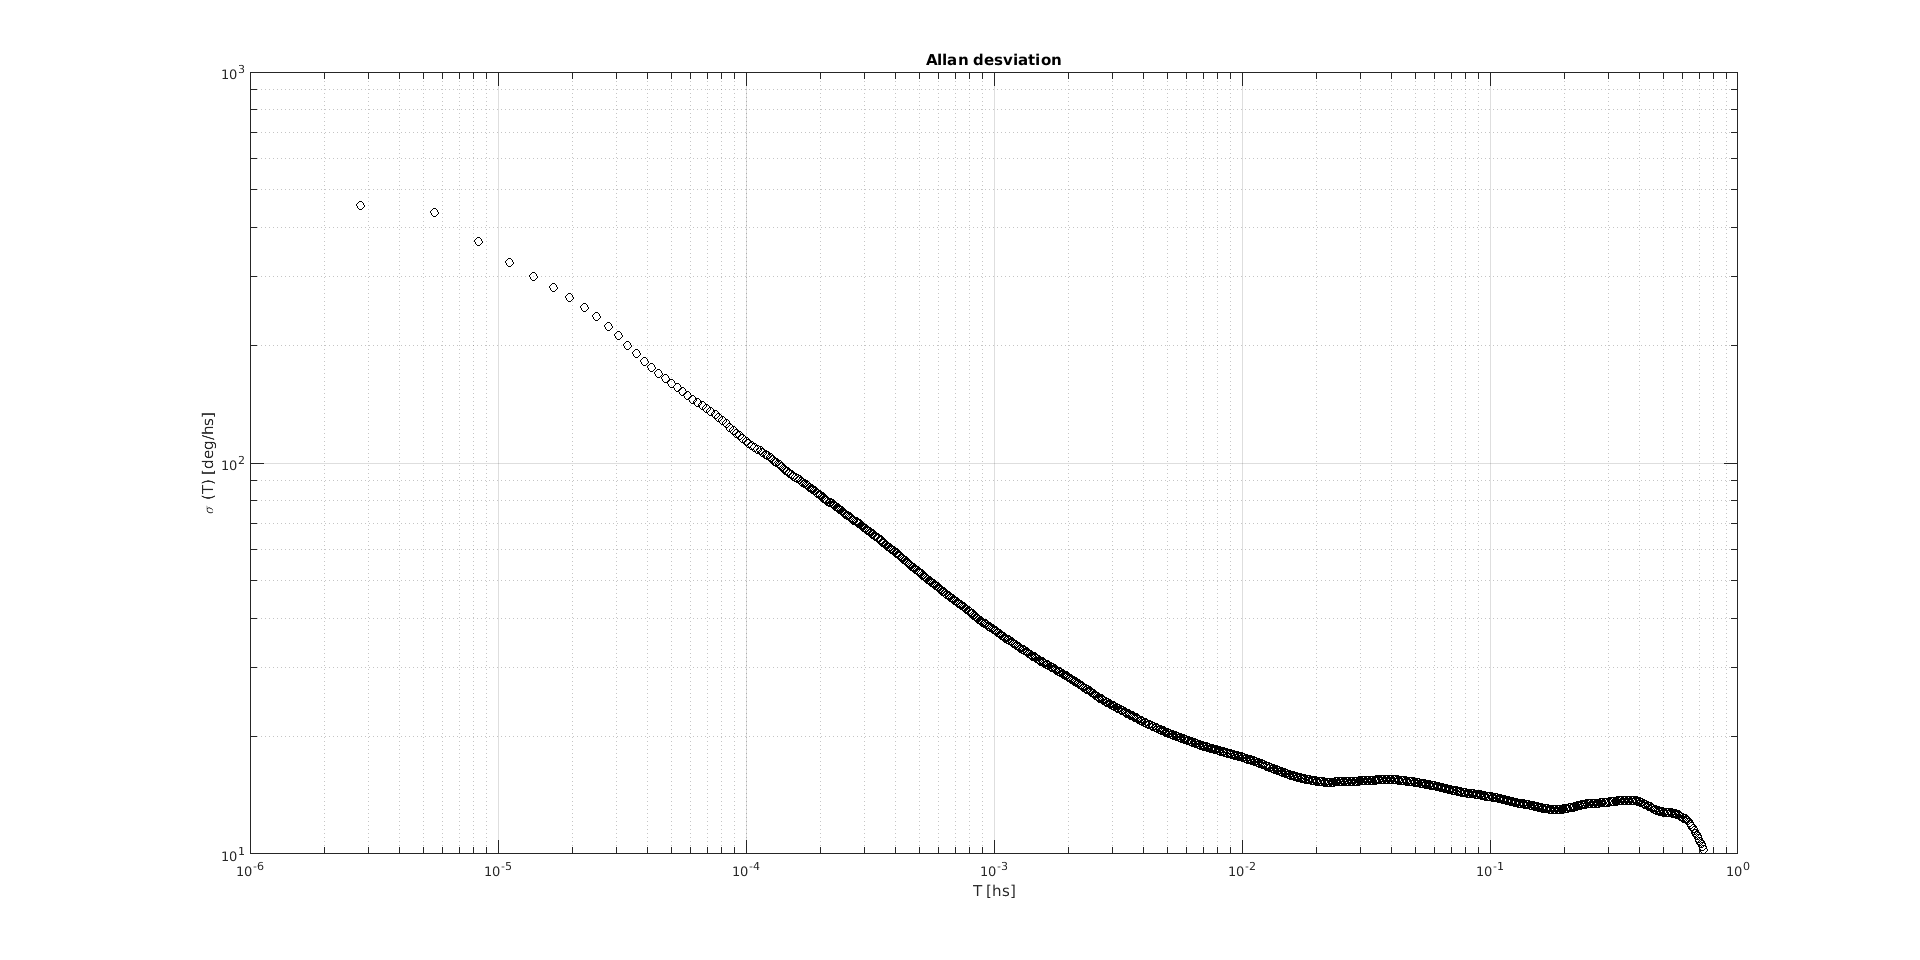
\includegraphics[width=8cm]{Figuras/AllanGyroy.png}
        \caption{Allan desviation: lecturas eje y}
        \label{fig:}
    \end{subfigure}%
    ~ 
    \caption{Lectura del eje y}
    \label{fig:lecturasEjey}
\end{figure*}
\begin{figure}[h!]
\centering
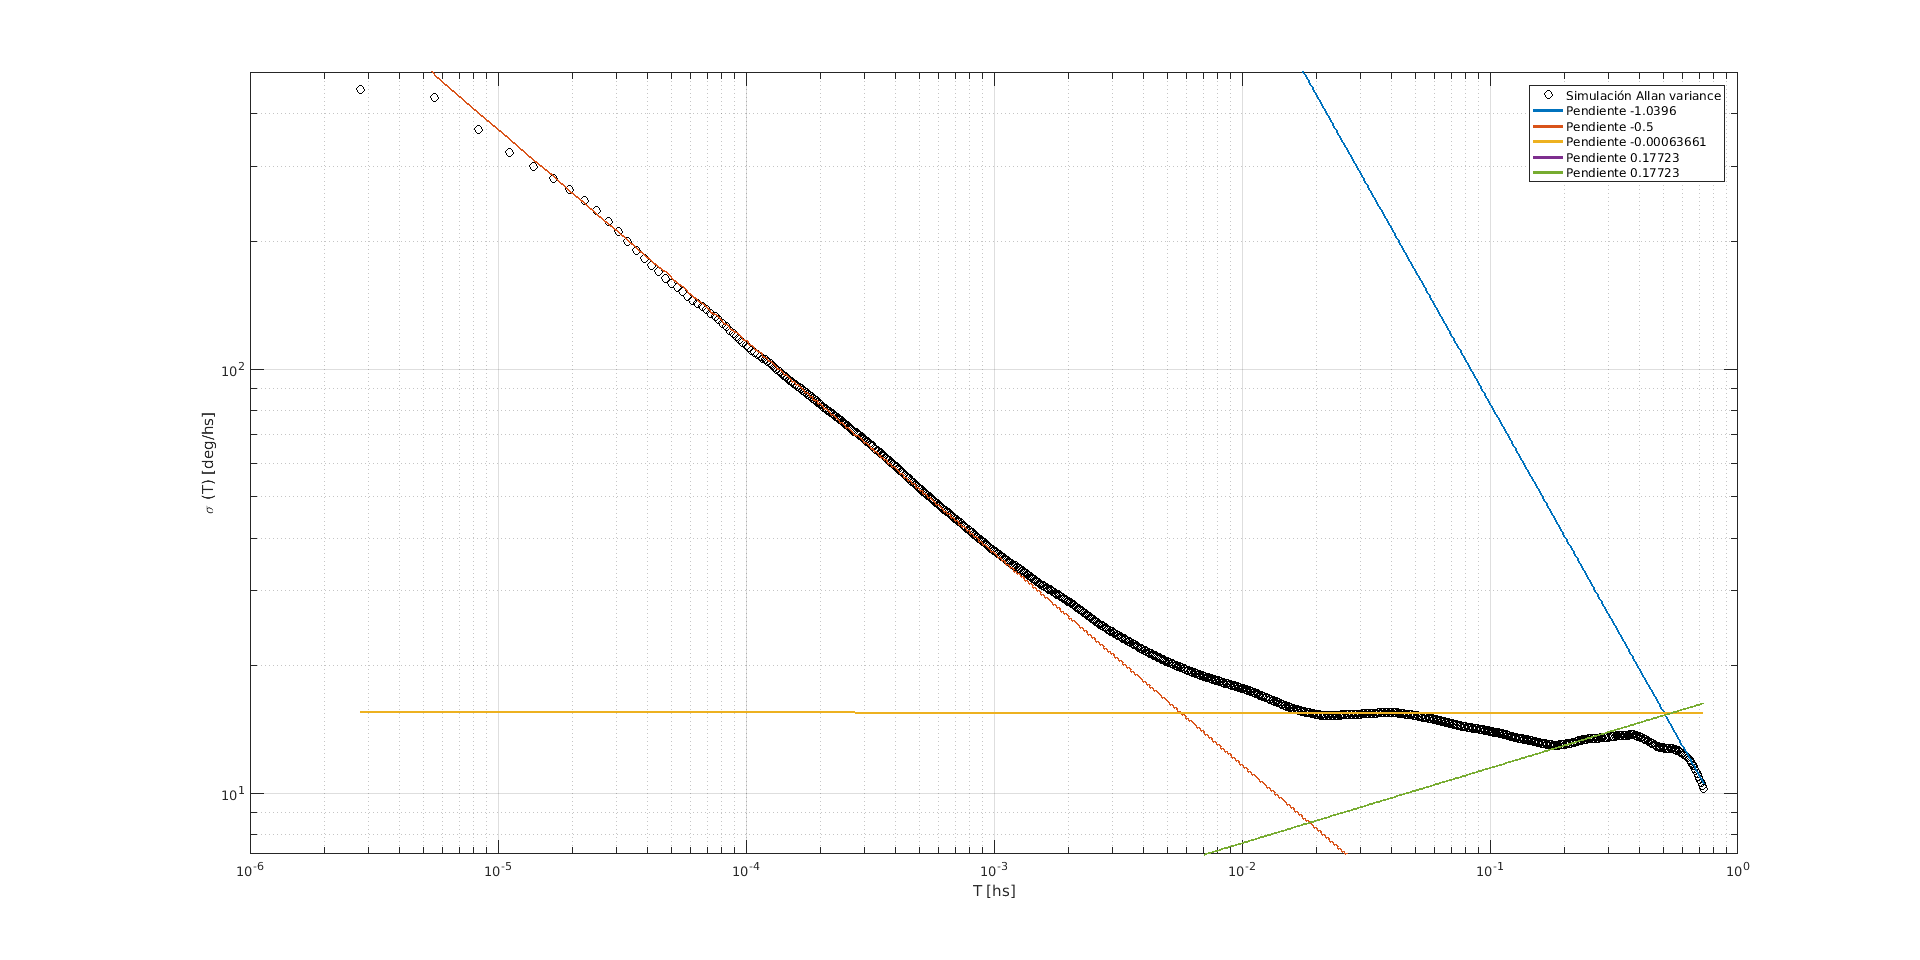
\includegraphics[width=8cm]{Figuras/AllanGyroyRectas.png}
\caption{Allan desviation del eje y junto con las rectas características}
\label{fig:lecturaEjeyRectas}
\end{figure}
\begin{figure*}[t!]
    \centering
    \begin{subfigure}[t]{0.5\textwidth}
        \centering
        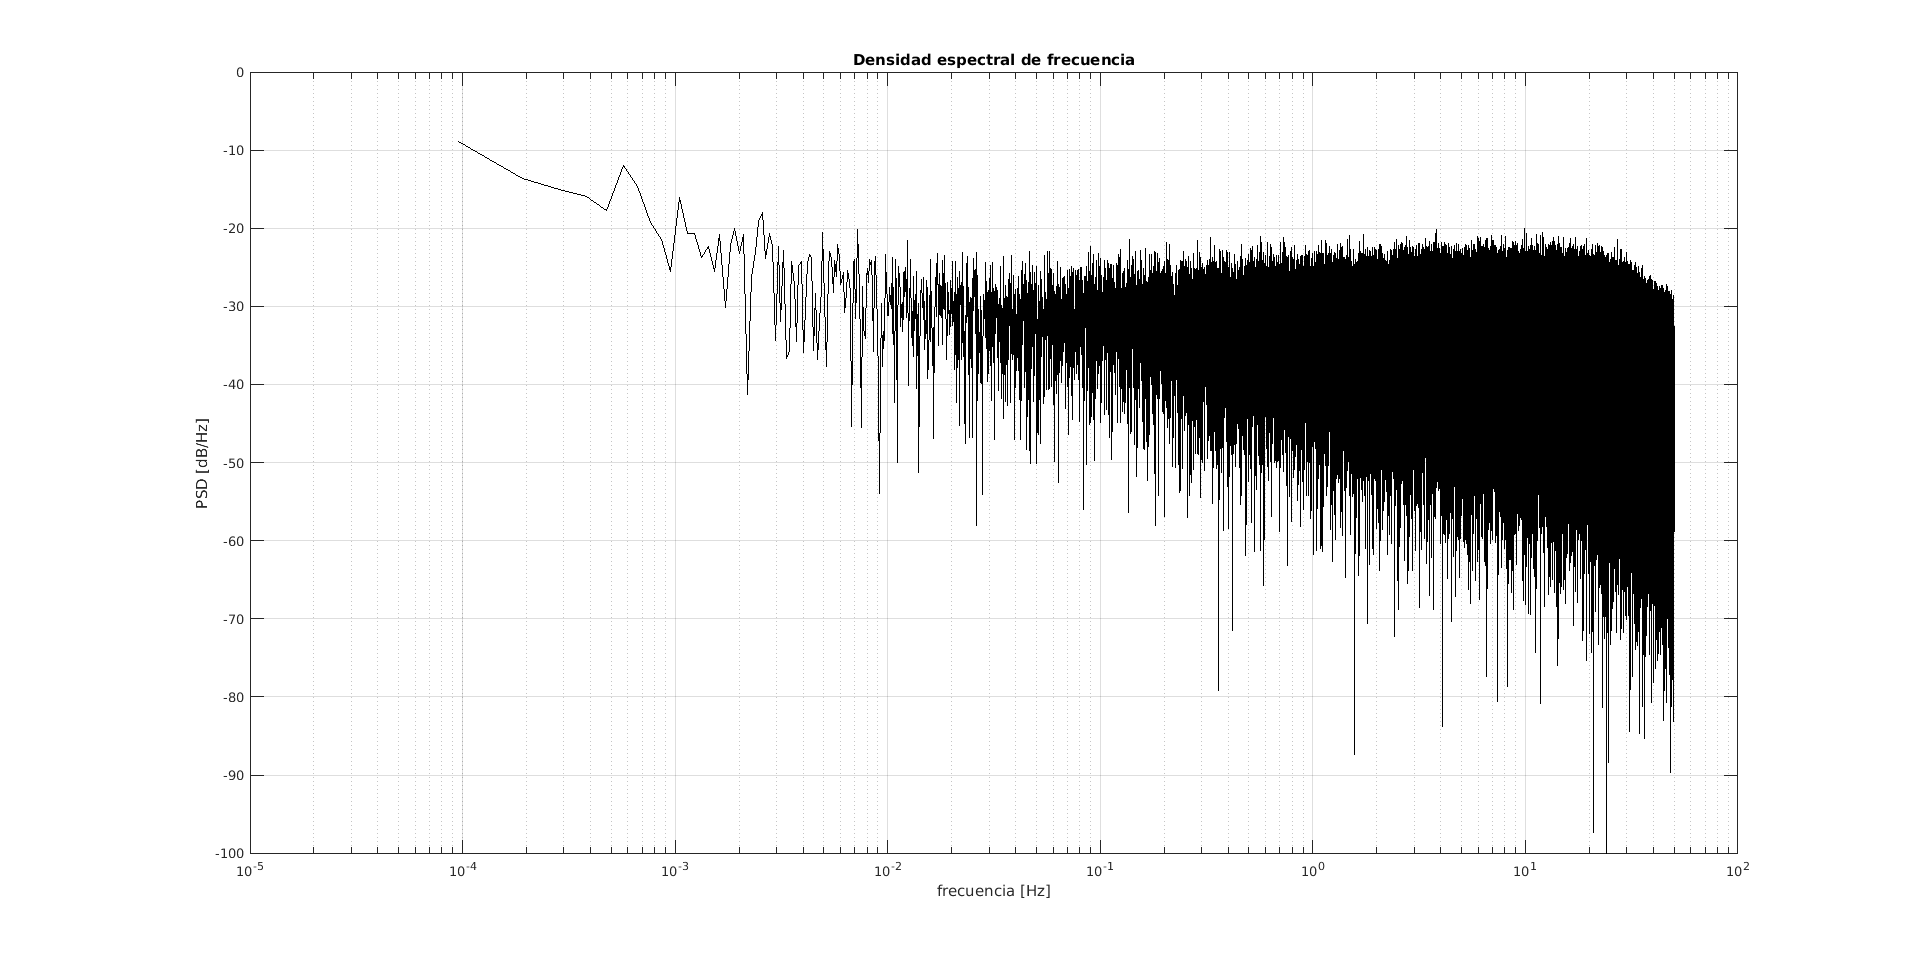
\includegraphics[width=8cm]{Figuras/PSDGyroz.png}
        \caption{PSD: lecturas eje z}
        \label{fig:}
    \end{subfigure}%
    \begin{subfigure}[t]{0.5\textwidth}
        \centering
        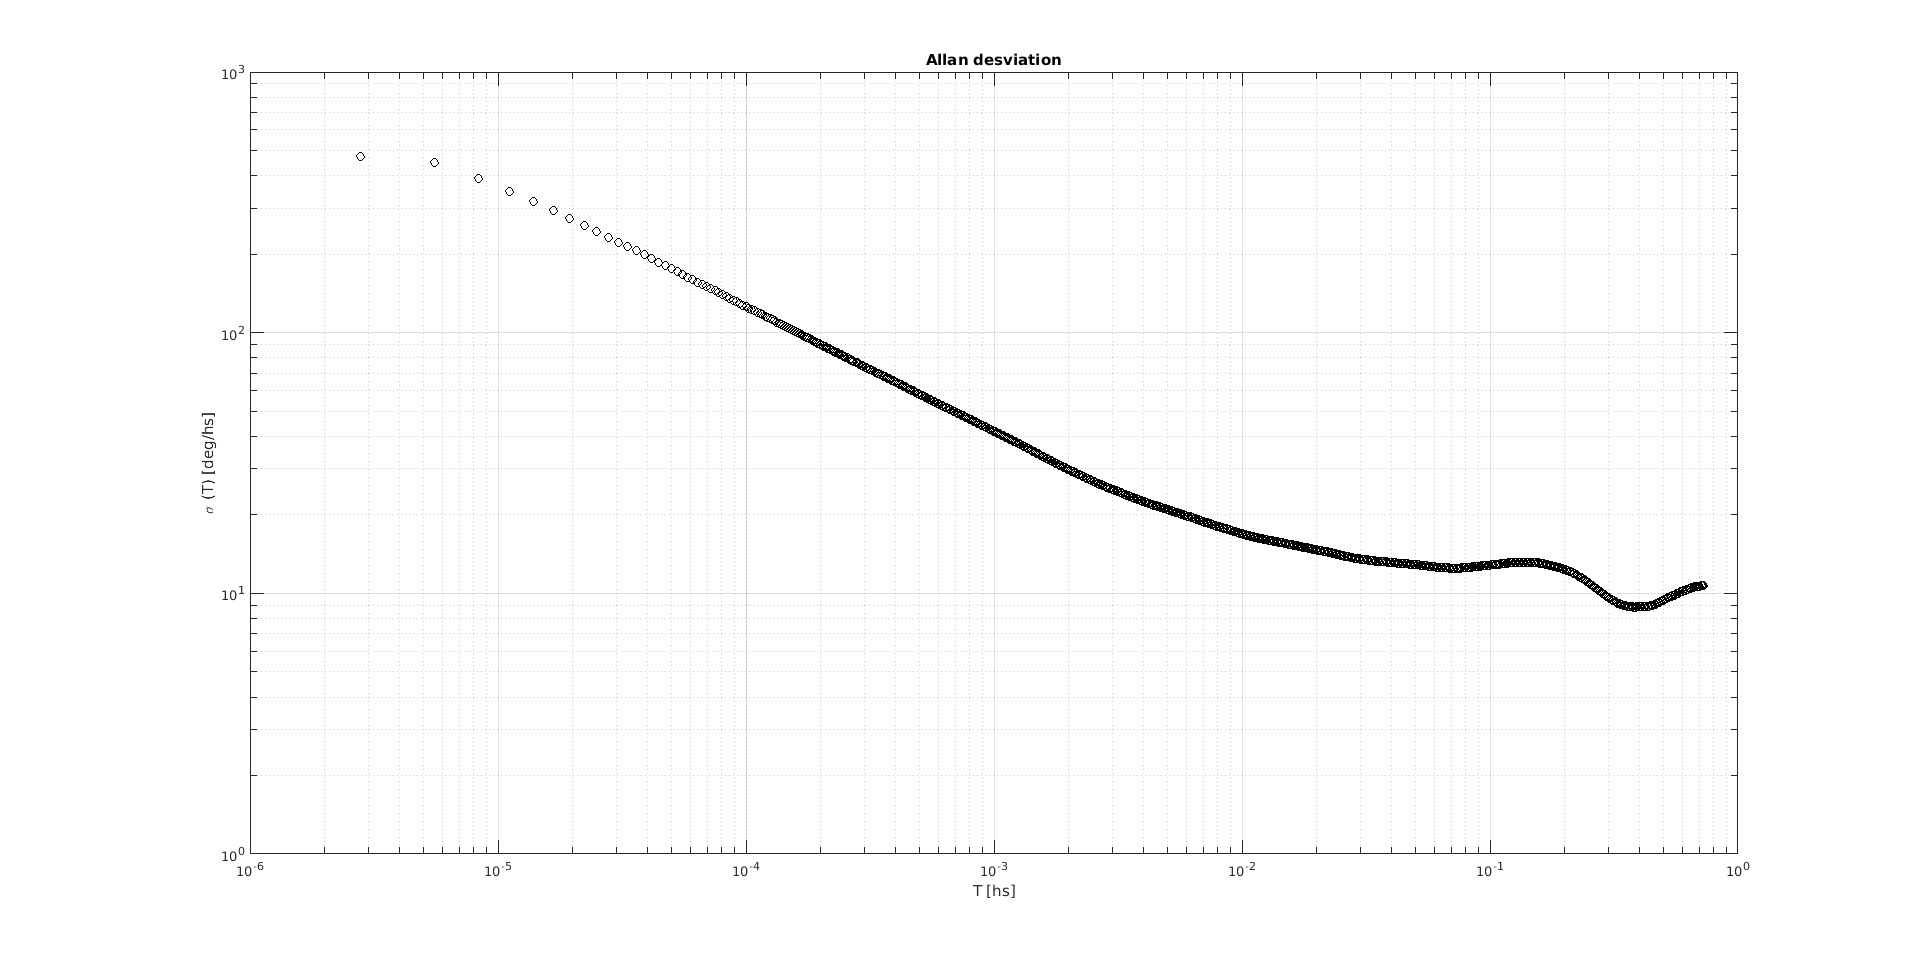
\includegraphics[width=8cm]{Figuras/AllanGyroz.png}
        \caption{Allan desviation: lecturas eje z}
        \label{fig:}
    \end{subfigure}%
    ~ 
    \caption{Lectura del eje z}
    \label{fig:lecturasEjez}
\end{figure*}
\begin{figure}[h!]
\centering
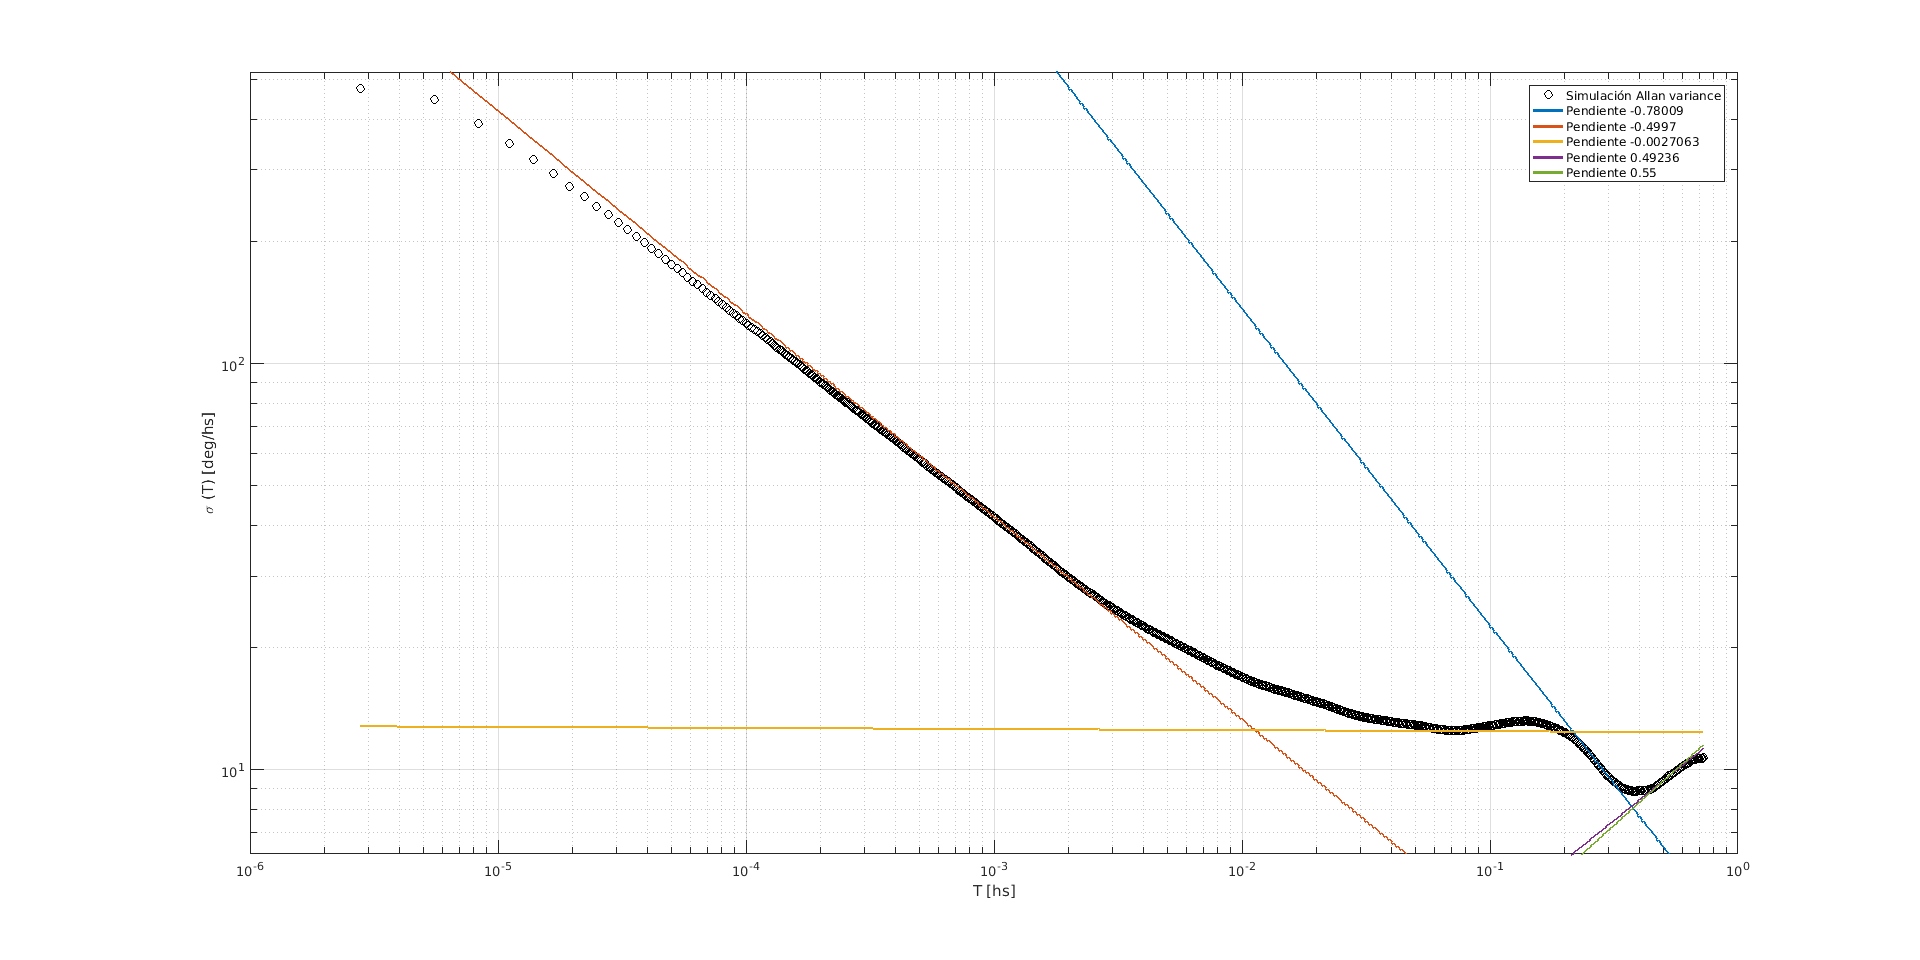
\includegraphics[width=8cm]{Figuras/AllanGyrozRectas.png}
\caption{Allan desviation del eje z junto con las rectas características}
\label{fig:lecturaEjezRectas}
\end{figure}
\begin{table}[h!]
\centering
\caption{Valores de los coeficientes registrados}
\label{tabla:valoresCoeficientesEjes}
\begin{tabular}{|c|c|c|c|c|}
\hline
Tipo de ruido&Coeficiente& Eje x & Eje y & Eje z \\ \hline
Quantization noise $\left[ deg\right]$&$Q_z$&$0.7528$&-&- \\ \hline
Angle random walk $\left[ deg/\sqrt{hs}\right]$&$Q$&$1.4$&-&-\\ \hline
Bias instability $\left[ deg/hs \right]$&$B$&$30.75$ &$23.34$ &$18.81$\\ \hline
%&&&&&& \\ \hline
\end{tabular}
\end{table}
%q
%Q
\section{CONCLUSIONES}
\newpage
\bibliographystyle{asmems4}
\bibliography{biblio}
\end{document}
%\begin{figure}[h!]
%\centering
%\includegraphics[width=8cm]{Figuras/.png}
%\caption{}
%\label{fig:}
%\end{figure}
%\begin{figure*}[t!]
%    \centering
%    \begin{subfigure}[t]{0.5\textwidth}
%        \centering
%        \includegraphics[width=8cm]{Figuras/.png}
%        \caption{}
%        \label{fig:}
%    \end{subfigure}%
%    \begin{subfigure}[t]{0.5\textwidth}
%        \centering
%        \includegraphics[width=8cm]{Figuras/.png}
%        \caption{}
%        \label{fig:}
%    \end{subfigure}%
%    ~ 
%    \caption{}
%    \label{}
%\end{figure*}
%\begin{table}[h!]
%\centering
%\caption{}
%\label{tabla:}
%\begin{tabular}{|c|c|c|}
%\hline
%
%%&&&&&& \\ \hline
%\end{tabular}
%\end{table}


%que